\documentclass[a5paper, 10pt, twoside, bahasa]{report}
\title{Tugas Akhir - Reidentifikasi Multi-Modal}
\usepackage{graphicx}
\usepackage{hyphenat}
\usepackage{comment}
\usepackage{array}
\usepackage{multirow}
\usepackage{rotating}
\usepackage{booktabs}
\usepackage[ruled,lined,commentsnumbered,linesnumbered]{algorithm2e}
\usepackage{algpseudocode}
\usepackage{makeidx}
\makeindex
\usepackage[pdfauthor={Charles Chang},bookmarksnumbered,pdfborder={0 0 0}]{hyperref}  
\usepackage[indonesian]{babel}
\usepackage{epsfig}
\usepackage{subfig}
\usepackage[top=25mm,left=25mm,right=20mm,bottom=25mm]{geometry}
\usepackage{pdflscape}
\usepackage{setspace}  
\usepackage{type1cm}
\usepackage{lettrine}
\usepackage{hyperref}
\usepackage[pageref]{backref}
\usepackage{multirow}
\usepackage{fancyhdr} 		% Untuk pengaturan header dan footer yang lebih kompleks
\usepackage{etoolbox} 		% Untuk melakukan perubahan (patch) command internal LaTeX
\usepackage{url}
\usepackage{longtable}
\usepackage{float}
\floatstyle{boxed}
\newfloat{program}{thp}{lop}
\floatname{program}{Program}
\usepackage[fleqn]{amsmath}
\usepackage{enumitem}
\usepackage{nonfloat}
\usepackage{ulem}
\usepackage[final]{pdfpages}
\usepackage [raggedright]{titlesec}

\usepackage{array}
\usepackage{multicol}
\usepackage{listings}
\usepackage{wrapfig}

% Caption label bold
\usepackage[labelfont=bf]{caption}
\captionsetup{labelfont=bf}

% Jarak caption dengan obyek
\captionsetup[figure]{font=small,skip=5pt}
\captionsetup[table]{font=small,skip=5pt}
\captionsetup[lstlisting]{font=small,skip=5pt}

% Caption nama
\renewcommand{\figurename}{Gambar}
\renewcommand{\tablename}{Tabel}
\renewcommand{\lstlistingname}{Kode}

% Buat source code
\usepackage{courier}
\lstset{
	% language=C++, 						% Bahasa pengrograman yang digunakan
	basicstyle=\ttfamily \footnotesize,	% Jenis font dalam listing & Ukuran font
	% numbers=left, 						% Posisi angka untuk line-number
	% numberstyle=\footnotesize, 		% Ukuran angka untuk line-numbers
	% stepnumber=1, 						% Jarak setiap line-numbers
	% numbersep=5pt, 					% Ukuran line-numbers
	backgroundcolor=\color{white}, 		% Warna background. Gunakan \usepackage{color} dulu
	showspaces=false, 					% Show spaces adding particular underscores
	showstringspaces=false, 				% Underline spaces within strings
	showtabs=false, 						% Show tabs within strings adding particular underscores
	frame=single, 						% Tambahkan Frame
	framesep=0.1pt,						% Jarak frame dengan list content keseluruhan
	framexbottommargin=4pt,				% Jarak frame dengan list content bawah
  	framextopmargin=4pt,					% Jarak frame dengan list content atas
  	framexleftmargin=0pt,				% Jarak frame dengan list content kiri
  	framexrightmargin=0pt,				% Jarak frame dengan list content kanan
	tabsize=2, 							% Sets default tabsize to 2 spaces
	captionpos=b,						% Posisi caption
	breaklines=true, 					% Line breaking
	breakatwhitespace=false, 			% Sets if automatic breaks should only happen at whitespace
	escapeinside={\%*}{*)}				% if you want to add a comment within your code
}

% Untuk cek nomor halaman
\usepackage{changepage}
\usepackage{graphicx}

%Untuk check mark dan x-mark
\usepackage{amssymb}% http://ctan.org/pkg/amssymb
\usepackage{pifont}% http://ctan.org/pkg/pifont
\newcommand{\cmark}{\ding{51}}%
\newcommand{\xmark}{\ding{55}}%

\usepackage{lipsum}
\hyphenation{meng-gerak-kan mem-per-kenal-kan me-nger-ja-kan sa-ran seg-men be-ru-pa rasp-ber-ry meng-hu-bun-kan ter-sim-pan smart-phone me-nya-ma-kan sin-kro-ni-sa-si ke-ce-pa-tan di-hu-bung-kan sam-bu-ngan me-ru-pa-kan meng-gu-na-kan ber-da-sar-kan di-la-ku-kan di-gu-na-kan di-ban-ding-kan}

% Definisi untuk "halaman sengaja dikosongkan"
\def\kosong{
  \vspace*{\fill}
  \begin{center}\textit{Halaman ini sengaja dikosongkan}\end{center}
  \vfill
}
\patchcmd{\cleardoublepage}{\hbox{}}{\kosong}{}{}

% Tambahkan PDF atau Gambar
\newif\ifpdf
\ifx\pdfoutput\undefined
   \pdffalse
\else
   \pdfoutput=1
   \pdftrue
\fi
\ifpdf
   \usepackage{graphicx}
   \usepackage{epstopdf}
   \DeclareGraphicsRule{.eps}{pdf}{.pdf}{`epstopdf #1}
   \pdfcompresslevel=9
\else
   \usepackage{graphicx}
\fi

% utk itemize yg lebih rapat
\newenvironment{packed_enum}{
\begin{enumerate}[nolistsep]
  \setlength{\itemsep}{0pt}
  \setlength{\parskip}{0pt}
  \setlength{\parsep}{0pt}
}{\end{enumerate}}

% Untuk citation
\newcommand{\tab}[1]{\hspace{.2\textwidth}\rlap{#1}}
\renewcommand*{\backreflastsep}{, }
\renewcommand*{\backreftwosep}{, }
\renewcommand*{\backref}[1]{}
\renewcommand*{\backrefalt}[4]{
  \ifcase #1
    No citations.
  \or
    (Dikutip pada halaman #2).
  \else
    (Dikutip pada halaman #2).
  \fi
}

% Pengaturan penomoran halaman menggunakan package fancyhdr
\fancyhf{} 								% Mengosongkan header dan footer
\renewcommand{\headrulewidth}{0pt} 		% Menghapus garis horizontal pada header
\pagestyle{fancy} 						% Mengubah pagestyle dokumen menjadi fancy
\fancyfoot[CE,CO]{\thepage}				% Footer kanan pada hal. ganjil dan sebaliknya
\patchcmd{\chapter}{plain}{fancy}{}{} 	% Mengubah pagestyle pada chapter menjadi fancy
\patchcmd{\chapter}{empty}{plain}{}{}

% Pengaturan format Chapter dan Section
\titleformat{\chapter}[display]{\bfseries\Large}{BAB \centering\thechapter}{0ex}{\vspace{0ex}\centering}[\vspace{0ex}]
\titleformat{\section}{\bfseries\large}{\MakeUppercase{\thesection}}{1ex}{}
\titlespacing*{\chapter}{0pt}{-4ex}{0pt}
\titlespacing{\section}{0pt}{0pt}{0pt}

\begin{document}
\pagenumbering{roman}
\singlespacing
\includepdf[pages=-, offset=0 0]{file/COVER-BUKU.pdf}
\includepdf[pages=-, offset=0 0]{file/Pengesahan.pdf}


% Abstrak bahasa indonesia
\addcontentsline{toc}{chapter}{Abstrak}
\begin{center}
\Large\textbf{ABSTRAK}
\end{center}
\vspace{1ex}

\begin{adjustwidth}{-0.2cm}{}
\begin{tabular}{lcp{0.6\linewidth}}
Nama Mahasiswa &:& Charles Chang \\
Judul Tugas Akhir &:& Re-identifikasi Orang menggunakan
Lightweight Convolutional Neural Network
pada Multi-Modal Image\\
Pembimbing &:& 1. Dr. Reza Fuad Rachmadi, S.T., M.T. \\
& & 2. Dr. I Ketut Eddy Purnama, S.T, M.T.  \\
\end{tabular}
\end{adjustwidth}
\vspace{1ex}

\setlength{\parindent}{0cm} Sebagai alat pelengkap keamanan, sistem CCTV semakin banyak digunakan di setiap ruang publik untuk memantau dan menganalisa tindakan kriminal pada suatu lokasi. Akan tetapi, pencarian kriminal secara manual masih rentan akan kesalahan manusia. Salah satu solusi membuat pencarian kriminal lebih efektif dan efisien adalah dengan penggunaan Re-identifikasi.
\par  Re-identifikasi merupakan sebuah teknik visi komputer dan deep learning dimana dilakukan pencarian ulang citra atau video milik sebuah identitas.Pada tugas akhir ini, akan dipelajari metode Re-identifikasi orang dengan citra multi-modal, adapun data Input yang akan digunakan berupa sketsa tubuh yang digambar oleh beberapa seniman berbeda.
\par  Teknik yang dipelajari akan diimplementasikan menggunakan Lightweight Convolutional Neural Network dan pre-trained weights dari model yang digunakan untuk mengklasifikasi dataset CIFAR-10. Hasil yang diharapkan melalui Tugas Akhir ini adalah terciptanya sebuah model yang dapat melakukan Re-identifikasi orang riil dari input sketsa menggunakan Lightweight Convolutional Neural Network, sehingga pencarian kriminal di Indonesia dapat dilakukan dengan lebih efisien.

\vspace{2ex}

Kata Kunci : Re-identifikasi, Multi-Modal, Kriminal
\newpage
\cleardoublepage

% Abstrak bahasa ingris
%\addcontentsline{toc}{chapter}{Abstract}
%\begin{center}
\Large\textbf{ABSTRACT}
\end{center}
\vspace{1ex}

\begin{adjustwidth}{-0.2cm}{}
\begin{tabular}{lcp{0.6\linewidth}}
\textit{Name} &:& Nama\\
\textit{Title} &:& \textit{Title} \\
\textit{Advisors} &:& 1. Pembimbing1 \\
& & 2. Pembimbing2 \\
\end{tabular}
\end{adjustwidth}
\vspace{1ex}

	\setlength{\parindent}{0cm} Explain
	\vspace{2ex}
	
	\textit{Keywords : Train, Digital Map, Path Index, Speed Limit, Early Warning}
	\newpage

%\cleardoublepage

% Kata pengantar
\addcontentsline{toc}{chapter}{KATA PENGANTAR} % kata pengantar
\begin{center}
\Large\textbf{KATA PENGANTAR}
\end{center}
\vspace{1ex}

\setlength{\parindent}{0.9cm} Puji dan syukur kehadirat Tuhan Yang Maha Esa atas segala karunia-Nya, penulis  dapat menyelesaikan penelitian ini dengan judul \textbf{Re-identifikasi Orang menggunakan Lightweight Convolutional Neural Network pada Multi-Modal Image}.
\vspace{1ex}

Penelitian ini disusun dalam rangka pemenuhan bidang riset di Departemen Teknik Komputer ITS, Bidang Studi \textit{Telematika}, serta digunakan sebagai persyaratan menyelesaikan pendidikan  S1. Oleh karena itu, penulis mengucapkan terima kasih kepada:
\vspace{1ex}

\begin{enumerate}[nolistsep]
  \item Tuhan Yang Maha Esa
  \item Orang tua saya, atas semangat dan segala dukungan yang telah diberikan
  \item Bapak Dr. Reza Fuad Rachmadi, S.T., M.T.
  \item Bapak Dr. I Ketut Eddy Purnama, S.T, M.T.
  \item Bapak-ibu dosen pengajar Departemen Teknik Komputer, atas pengajaran, bimbingan, serta perhatian yang diberikan kepada penulis selama ini.
  \item Serta teman - teman angkatan 2017 yang telah bersama - sama melalui kehidupan perkuliahan bersama penulis
\end{enumerate}
\vspace{1ex}

Kesempurnaan hanya milik Tuhan Yang Maha Esa, untuk itu penulis memohon segenap kritik dan saran yang  membangun. Semoga penelitian ini dapat memberikan manfaat bagi kita semua. Amin.
\begin{flushright}
\begin{tabular}[b]{c}
  Surabaya, April 2021
  \\
  \\
  Penulis
\end{tabular}
\end{flushright}
\cleardoublepage

% Daftar isi
\renewcommand*\contentsname{DAFTAR ISI}
\addcontentsline{toc}{chapter}{\contentsname}
\titlespacing*{\chapter}{0pt}{-4ex}{2ex}
\tableofcontents	
\cleardoublepage

% Daftar gambar
\renewcommand*\listfigurename{DAFTAR GAMBAR}
\addcontentsline{toc}{chapter}{\listfigurename}
\titlespacing*{\chapter}{0pt}{-4ex}{2ex}
\listoffigures
\cleardoublepage

% Daftar tabel
\renewcommand*\listtablename{DAFTAR TABEL}
\addcontentsline{toc}{chapter}{\listtablename}
\titlespacing*{\chapter}{0pt}{-4ex}{2ex}
\listoftables
\cleardoublepage

% Nomenklatur
\addcontentsline{toc}{chapter}{NOMENKLATUR}
\begin{center}
	\Large\textbf{NOMENKLATUR}
\end{center}
\vspace{1ex}

\begin{tabular}{c m{30em}}
	$fps$	& : \textit{Frame Per Second} / Jumlah Citra Perdetik\\
	$unit$	& : unit pengukuran \textit{Unity Game Engine} \\
	
	
\end{tabular}
\vspace{1ex}
\cleardoublepage

% BAB isi buku
\titleformat{\chapter}[display]{\bfseries\Large}{BAB \centering\thechapter}{0ex}{\vspace{0ex}\centering}[\vspace{0ex}]
\titleformat{\section}{\bfseries\large}{\MakeUppercase{\thesection}}{1ex}{}
\titleformat{\subsection}{\bfseries\large}{\MakeUppercase{\thesubsection}}{1ex}{}
\titleformat{\subsubsection}{\bfseries\large}{\MakeUppercase{\thesubsubsection}}{1ex}{}
\titlespacing*{\chapter}{0pt}{-4ex}{0pt}
\titlespacing{\section}{0pt}{0pt}{0pt}
\titlespacing{\subsection}{0pt}{0pt}{0pt}
\titlespacing{\subsubsection}{0pt}{0pt}{0pt}

% Indent paragraph
\setlength{\parindent}{0.8cm}

% Penambahan halaman kosong otomatis
\chapter{PENDAHULUAN}
\pagenumbering{arabic}
\vspace{1ex}

\section*{}
Penelitian ini di latar belakangi oleh berbagai kondisi yang menjadi acuan. Selain itu juga terdapat beberapa permasalahan yang akan dijawab sebagai luaran dari penelitian.
\vspace{1ex}

\section{Latar belakang}
\vspace{1ex}

Saat ini teknologi telah berkembang pesat sehingga penggunaan kamera pengawasan atau \textit{CCTV} sudah umum dipakai. Hasil rekaman dari kamera ini  merupakan informasi visual yang sangat vital dan dapat berperan sebagai saksi terjadinya tindakan kriminal. Hasil rekaman ini mempunyai peran penting dalam memberikan bukti di investigasi kriminal dan perselisihan.  
\vspace{1ex}

Pada tahun 2021 ini, Indonesia merupakan negara dengan jumlah penduduk terpadat ke-4 di dunia, dimana pada DKI Jakarta sendiri terdapat 10.4 juta penduduk, yaitu sekitar 333\% lebih banyak dibanding Surabaya \cite{cit:1, cit:2}. Dari data yang diambil dari Badan Pusat Statistik, Polda Metro Jaya mencatat jumlah kejahatan terbanyak yaitu 31.934 kejadian, dan pada tahun 2020 ini terlihat trend adanya peningkatan tindak kriminal di seluruh Indonesia \cite{cit:3, cit:4, cit:5, cit:6}. Fakta – fakta inilah yang mendorong riset – riset mengenai pengurangan angka kriminalitas dengan berbagai macam cara, dibutuhkan adanya otomasi yang dapat mengurangi biaya dan beban kerja pihak kepolisian.
\vspace{1ex} 
 
Re-identifikasi manusia merupakan sebuah teknik visi komputer dan deep learning dimana pada sebuah lingkungan yang terdapat beberapa kamera pengawas dilakukan adanya pencocokan citra seseorang, kepada citra yang ditangkap pada kamera lain. Masalah utama yang ditangani oleh Re-identifikasi manusia dapat disimpulkan sebagai cara untuk mencari representasi diskriminatif milik individu yang ingin dicari. Dengan membuat sistem re-identifikasi manusia, pemeriksaan hasil rekaman yang dilakukan oleh pihak kepolisian dapat dilakukan dengan jauh lebih cepat, dan dapat menekan biaya yang digunakan untuk membayar tenaga kerja. Tidak hanya  untuk melakukan pencarian pelaku tindak kriminal, re-identifikasi dapat digunakan juga untuk melihat apakah barang yang tertinggal pada suatu lokasi diambil individu yang sama, dan dapat membantu pihak sekuriti mencari orang yang hilang. Re-identifikasi manusia dapat mempermudah aktivitas - aktivitas yang sebelumnya dilakukan secara manual, maka dari itu pencarian individu sangat dibutuhkan dengan menggunakan teknologi \textit{machine learning} untuk mempercepat proses yang sebelumnya memakan waktu yang sangat lama.
\vspace{1ex} 

\section{Permasalahan}
\vspace{1ex}
Berdasarkan data yang telah dipaparkan di latar belakang, dapat dirumuskan beberapa rumusan masalah sebagai berikut:
\begin{enumerate}
	\vspace{-1.3mm}
	\item Indonesia merupakan negara dengan penduduk ke-empat terbanyak di dunia sehingga pencarian pelaku tindak kriminal diantara penduduk sipil sulit untuk dilakukan.
	\vspace{-2mm}
	\item Data hasil rekaman kamera masih diperiksa secara manual oleh pihak kepolisian sehingga waktu dan ketepatan pencarian masih tidak optimal.
\end{enumerate}

\section{Tujuan}
\vspace{1ex}

Adapun tujuan dari penelitian Tugas Akhir ini adalah mengembangkan model re-identifikasi orang menggunakan \textit{Lightweight Convolutional Neural Network} untuk mengindentifikasi ulang seseorang yang tertangkap pada beberapa \textit{CCTV} berbeda dengan menggunakan sketsa dari beberapa seniman sebagai input.

\vspace{1ex}

\section{Batasan masalah}
\vspace{1ex}
Batasan masalah yang timbul dari permasalahan Tugas Akhir ini adalah:
\vspace{1ex}
\begin{enumerate}
	\vspace{-2mm}
	\item Data \textit{training} dan \textit{testing} menggunakan data yang diambil dari PKU SketchRe-ID Dataset.
	\vspace{-2mm}
	\item Jenis re-identifikasi orang yang akan dilakukan adalah \textit{Closed Set} dan \textit{Short Term}.
	\vspace{-2mm}
	\item Training akan dilakukan menggunakan \textit{Lightweight Convolutional Neural Network}
\end{enumerate}
\vspace{1ex}

\section{Sistematika Penulisan}
\vspace{1ex}
Laporan penelitian Tugas Akhir ini disusun dalam sistematika yang terstruktur, sehingga mudah dipahami dan dipelajari oleh pembaca maupun seseorang yang ingin melanjutkan penelitian ini. Alur sistematika penulisan laporan penelitian ini yaitu sebagai berikut:
\vspace{1ex}

\begin{enumerate}[nolistsep]
	\item BAB I Pendahuluan

	Bab ini berisi uraian tentang latar belakang permasalahan, penegasan dan alasan pemilihan judul, sistematika laporan, tujuan dan metodologi penelitian.
	\vspace{1ex}

	\item BAB II Dasar Teori

	Bab ini berisi tentang uraian secara sistematis teori-teori yang berhubungan dengan permasalahan yang dibahas pada penelitian ini. Teori-teori ini digunakan sebagai dasar dalam penelitian, yaitu sistem simulator dan pengambilan data variabel - variabel uji.
	\vspace{1ex}

	\item BAB III Perancangan Sistem dan Impementasi

	Bab ini berisi tentang penjelasan-penjelasan terkait eksperimen yang akan dilakukan dan langkah-langkah pengolahan data hingga menghasilkan visualisasi. Guna mendukung eksperimen pada penelitian ini, digunakanlah blok diagram atau \textit{work flow} agar penjelasan sistem yang akan dibuat dapat terlihat dan mudah dibaca untuk implementasi pada pelaksanaan tugas akhir.
	\vspace{1ex}

	\item BAB IV Pengujian dan Analisa

	Bab ini menjelaskan tentang pengujian eksperimen yang dilakukan terhadap data dan analisanya. Beberapa teknik visualisasi akan ditunjukan hasilnya pada bab ini dan dilakukan analisa terhadap hasil visualisasi dan informasi yang didapat dari hasil mengamati visualisasi yang tersaji
	\vspace{1ex}

	\item BAB V Penutup

	Bab ini merupakan penutup yang berisi kesimpulan yang diambil dari penelitian dan pengujian yang telah dilakukan. Saran dan kritik yang membangun untuk pengembangkan lebih lanjut juga dituliskan pada bab ini.
\end{enumerate}
\vspace{1ex}

\section{Relevansi}
\begin{enumerate}
    \item Lightweight Residual Network for Person Re-Identification (Reza Fuad Rachmadi, Supeno Mardi Nugroho, I Ketut Eddy Purnama) \cite{cit:14}
    \par
	\textit{Lightweight Residual Network for Person Re-Identification} ini merupakan sebuah implementasi \textit{lightweight CNN} untuk melakukan re-Identifikasi manusia, lightweight CNN yang digunakan berbasis \textit{Residual Network} dengan menggunakan pre trained weights yang pernah  digunakan untuk memecahkan masalah klasifikasi CIFAR-10. Lightweight network dibuat dengan membuat \textit{ensemble} dari beberapa Residual Network lemah yang ada menghasilkan sebuah model yang lebih kuat. Berdasarkan hasil dari riset yang dilakukan, meskipun lightweight CNN tidak mendapatkan akurasi tercanggih dibandingkan model-model lainnya, banyak nya informasi yang didapatkan oleh model ini sangat tinggi, dan dapat dikatakan model ini lebih efisien dari model-model lainnya.
    \vspace{1ex}
    
    \item Torchreid: A Library for Deep Learning Person Re-Identification in Pytorch. (Kaiyang Zhou, Tao Xiang). \cite{cit:16}
    \par
	 Torchreid merupakan sebuah \textit{library deep learning} yang dibuat oleh Kaiyang Zhou untuk mempercepat implementasi dan percobaan re-identifikasi. Library ini secara umum dibuat dengan menggunakan bahasa Python dengan beberapa kode berbasis Cython untuk optimisasi. Pada library ini dataset sudah di \textit{preprocess} dan di implementasi sesuai dengan protokol evaluasi masing masing dataset sehingga dapat dibandingkan dengan penelitian lain yang terkait.
    \vspace{1ex}
    
    \item Adaptive L2 Regularization in Person Re-Identification. (Xingyang Ni, Liang Fang, Heikki Huttunen) \cite{cit:17}
    \par
    
    \textit{Adaptive L2 Regularization in Person Re-Identication} merupakan sebuah penelitian untuk menambahkan regularisasi L2, dimana faktor regularisasi dapat berubah ubah secara adaptif pada \textit{baseline} model. Dari hasil penelitan yang dilakukan regularisasi L2 secara adaptif dapat meningkatkan akurasi model sekitar 1 hingga 2\% untuk \textit{dataset} Market-1501, DukeMTMC dan MSMT17.
    \vspace{1ex}
    
    \item Cross-Domain Adversarial Feature Learning for Sketch
    Re-identification. (Lu Pang, Yaowei Wang, Yi-Zhe Song, Tiejun Huang, Yonghong Tian) \cite{cit:12}
    \par
    
    \textit{Cross-Domain Adversarial Feature Learning for Sketch Re-identification} merupakan penelitian yang pertama kali menggunakan gambar sketsa sebagai input dari model re-identifikasi manusia, namun dari model yang digunakan sendiri merupakan model yang telah di optimisasi untuk melakukan pengambilan informasi dari sketsa, seperti Triplet SN dan model GN Siamese yang merupakan gabungan dari dua cabang dari model GoogleNet yang dioptimisasi dengan menggunakan pairwise verification loss.
    \vspace{1ex}
    
    \par Dapat dilihat dari penelitian-penelitian terkait diatas, selain pada penelitian \textit{Cross-Domain Adversarial Feature Learning for Sketch Re-identification}, hal yang difokuskan adalah metode re-identifikasi pada gambar orang riil yang tertangkap pada CCTV menggunakan gambar lain dari individu tersebut. Sedangkan pada penelitian yang kami usulkan pada Tugas Akhir ini adalah untuk melakukan re-identifikasi pada gambar orang riil yang tertangkap pada CCTV menggunakan gambar sketsa \textit{full body}  sebagai \textit{input}.
    Selain itu penelitian yang dilakukan menggunakan model lightweight classical seperti ResNet, yang bukan merupakan fokus dari penelitian terakhir.

\end{enumerate}
\vspace{1ex}
\cleardoublepage
\chapter{TINJAUAN PUSTAKA}
\vspace{1ex}

\section*{}
Demi mendukung penelitian ini, dibutuhkan beberapa teori penunjang sebagai bahan acuan dan referensi. Dengan demikian penelitian ini menjadi lebih terarah. 
\vspace{1ex}

\section{Machine Learning}
\vspace{1ex}

\begin{figure} [!htb]
	\captionsetup{justification=centering}
	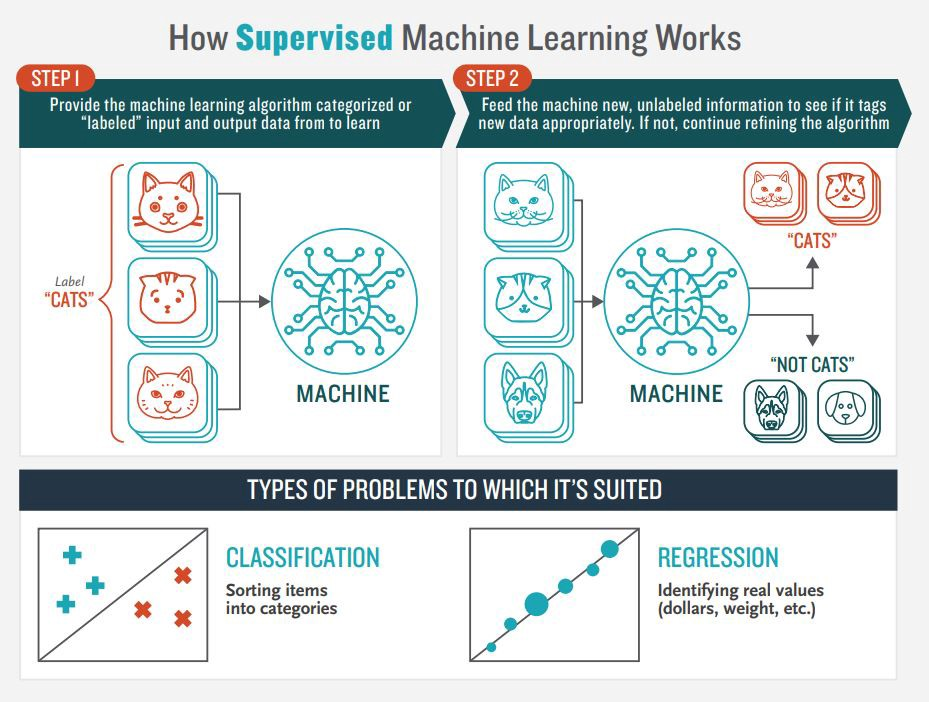
\includegraphics[scale=0.2]{img/supervised.jpeg}
	\caption{Cara Kerja Supervised Learning\cite{cit:8}}
	\label{fig:2.1}
\end{figure}

\textit{Machine learning} atau pembelajaran mesin adalah suatu cabang teknologi yang menerapkan penggunaan \textit{artificial intelligence}. \textit{Machine learning} pertama kali diperkenalkan oleh Thomas Bayes, Adrien-Marie Legendre, dan Andrey Markov pada sekitar tahun 1920\cite{cit:7}. Dengan menggunakan fundamental \textit{Machine Learning} yang diciptakan oleh ilmuwan - ilmuwan tersebut, \textit{Artificial Intelligence} kini dapat berkembang sampai dapat mengalahkan pemain catur profesional.
\vspace{1ex}

\par Dengan berkembangnya \textit{machine learning}, tugas-tugas yang dilakukan oleh \textit{machine learning} ini pun semakin beragam. Beberapa contoh dari tugas-tugas yang dapat dilakukan oleh \textit{Machine Learning} adalah validasi data, menemukan pola-pola tertentu dari sumber data yang besar, mengklasifikasi grup dan objek berdasarkan kesamaan pola.

\vspace{1ex}
\par \textit{Supervised learning} jika diartikan secara harfiah adalah pembelajaran yang ada supervisornya. Disini supervisi dilakukan oleh orang yang melakukan training kepada label di setiap datanya. Sebagai contoh dapat dilihat pada gambar 2.1. 
\vspace{1ex}

\par Pada gambar diatas, masing-masing gambar kucing diberi label “CATS” dan yang bukan kucing (“anjing”,”beruang”,”lain-lain”) diberi label “NOT CATS”. Ketika gambar baru dimasukkan setiap label akan dicompare sampai selesai, dan yang memiliki persentase lebih banyak akan diambil sebagai prediksi akhir.

\vspace{1ex}

\par Pada pendekatan \textit{supervised learning}, terdapat input dan output yang dapat dibuat menjadi hubungan matematis.\textit{Supervised learning} cocok untuk digunakan untuk memprediksi dimana sudah ada contoh data yang lengkap, sehingga pola yang terbentuk adalah hasil pembelajaran dari data lengkap tersebut. Beberapa algoritma yang termasuk dalam \textit{supervised learning} adalah sebagai berikut:
\begin{enumerate}
	\vspace{-2mm}
	\item Regresi Linier Berganda
	\vspace{-2mm}
	\item Analisis Deret Waktu
	\vspace{-2mm}
	\item \textit{Decision Tree} dan \textit{Random Forest}
	\vspace{-2mm}
	\item \textit{Naive Bayes Classifier}
	\vspace{-2mm}
	\item \textit{Nearest Neighbor Classifier}
	\vspace{-2mm}
	\item \textit{Artificial Neural Network}
	\vspace{-1mm}
\end{enumerate}
\par Jika dibandingkan dengan \textit{supervised learning}, \textit{unsupervised learning} tidak membutuhkan adanya label sebagai dasar prediksi melainkan menggunakan kesamaan atribut - atribut yang dimiliki oleh data tersebut. Jika atribut - atribut tersebut memiliki kesamaan maka data tersebut akan di \textit{cluster} menjadi satu. Sebagai contoh dapat dilihat pada gambar di bawah :

\begin{figure}[h!]
	\centering
	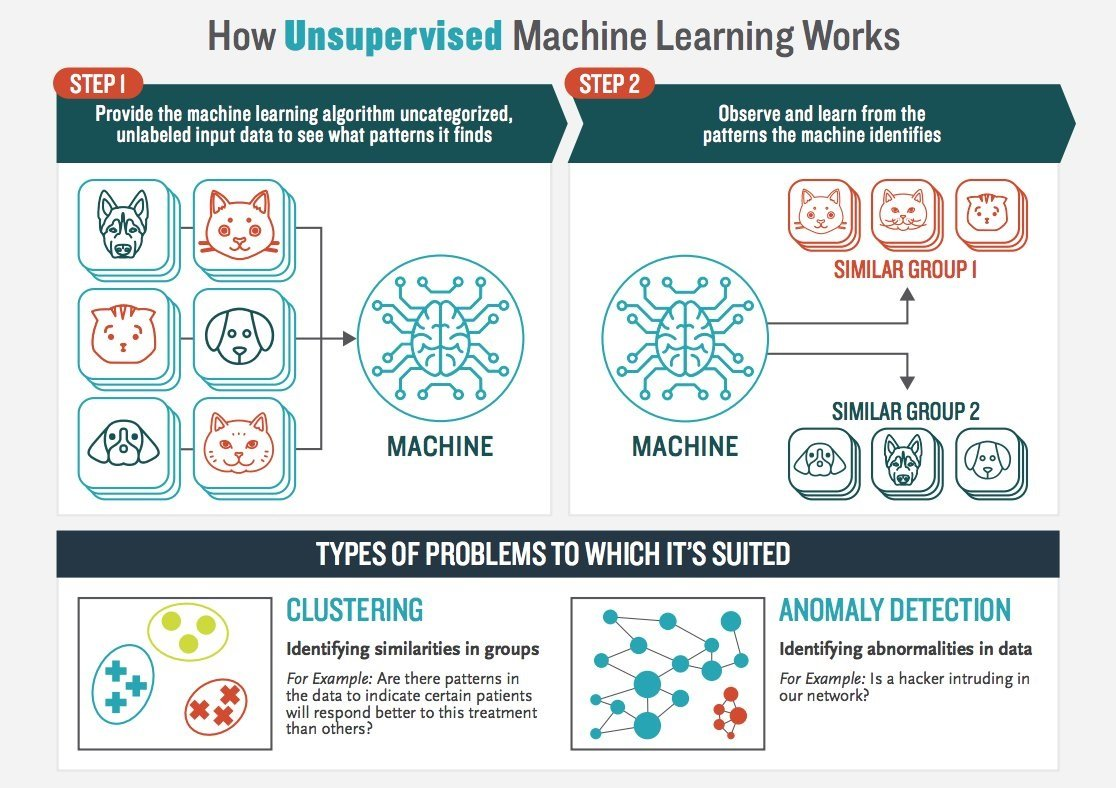
\includegraphics[scale=0.18]{img/unsupervised.jpg}
	\caption{Cara kerja Unsupervised Learning \cite{cit:8}}
	\label{fig:Unsupervised}
\end{figure}

\pagebreak

\par Pada Gambar 2.2 dapat dilihat bahwa disediakan gambar- gambar yang tidak memiliki label ke algoritma \textit{machine learning}. Setelah itu \textit{artificial intelligence} akan memisahkan gambar mana yang memiliki kesamaan di dalam \textit{cluster}. \textit{Cluster} yang ada merupakan hasil akhir klasifikasi yang dilakukan.

\par Namun \textit{unsupervised learning} tidak memiliki hasil spesifik layaknya pada \textit{supervised learning}. Hal ini dikarenakan tidak adanya label dasar (ground truth). Beberapa algoritma yang digunakan di \textit{unsupervised learning} :
\begin{enumerate}
	\vspace{-2mm}
	\item \textit{Clustering}
	\vspace{-2mm}
	\item \textit{Anomaly Detection}
	\vspace{-2mm}
	\item \textit{Training Model}
	\vspace{-2mm}
	\item \textit{Association Discovery}
\end{enumerate}

\vspace{1ex}

\par \textit{Deep learning} (Pembelajaran Dalam) merupakan bagian yang dalam dari \textit{machine learning} yang terdiri dari pemodelan fungsi yang ditata berlapis dan mendalam dengan menggunakan \textit{Artificial Neural Network} (ANN). ANN merupakan sebuah teknik atau pendekatan pengolahan informasi yang terinspirasi oleh cara kerja sistem saraf biologis, khususnya pada sel otak manusia dalam memproses informasi. Jenis pembelajaran dalam deep learning berupa \textit{supervised, semi-supervised}, dan \textit{unsupervised}.Deep learning dapat diimplementasikan dalam pengenalan citra, pengenalan suara, klasifikasi teks, dan sebagainya. 

\begin{figure}[h!]
\centering
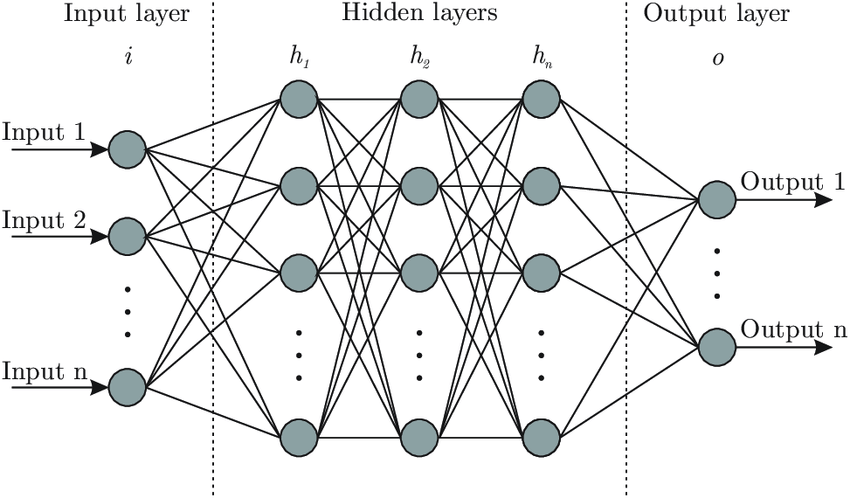
\includegraphics[scale=0.2]{img/Artificial.png}
\caption{Bentuk Artificial Neural Network \cite{cit:18}}
\label{fig:ANN}
\end{figure}

\section{\textit{Residual Network}}
\vspace{1ex}

\textit{Residual Neural Network} atau \textit{ResNet} merupakan sebuah \textit{Artificial Neural Network} (ANN) yang dibuat berdasarkan bentuk korteks serebral milik manusia. \textit{Residual Network} melakukan hal ini dengan memperkenalkan \textit{skip connection} atau \textit{shortcut}, dimana model dapat melompat dua atau tiga \textit{layer} jika memang hal tersebut merupakan hasil terbaik. Sebelum adanya model \textit{Residual Neural Network} penambahan layer pada suatu model hanya akan meningkatkan akurasi sampai suatu batas tertentu, sehingga penambahan layer setelah 20 hanya menambahkan kompleksitas model bukannya akurasi. Namun pada penelitian \textit{Deep Residual Learning for Image Recognition} yang dibuat oleh Kaiming He pada tahun 2015 memproposikan sebaliknya, apabila layer tambahan yang ada dapat mempelajari matriks identitas, maka minimal akurasi yang didapat pada \textit{layer} akan sama dengan apabila tidak menambahkan \textit{layer}. Untuk membuktikan hal tersebut dibuatlah sistem \textit{skip connection} atau \textit{shortcut} sehingga model dapat mempelajari matriks identitas dengan lebih mudah. Dari penelitian yang dilakukan pada dataset \textit{ImageNet}, \textit{Residual Network} dapat mengurangi \textit{loss} yang didapat ketika menambahkan lebih banyak \textit{layer} pada \textit{Artificial Neural Network} yang dibuat. \cite{cit:10}

\begin{figure}[h!]
	\centering
	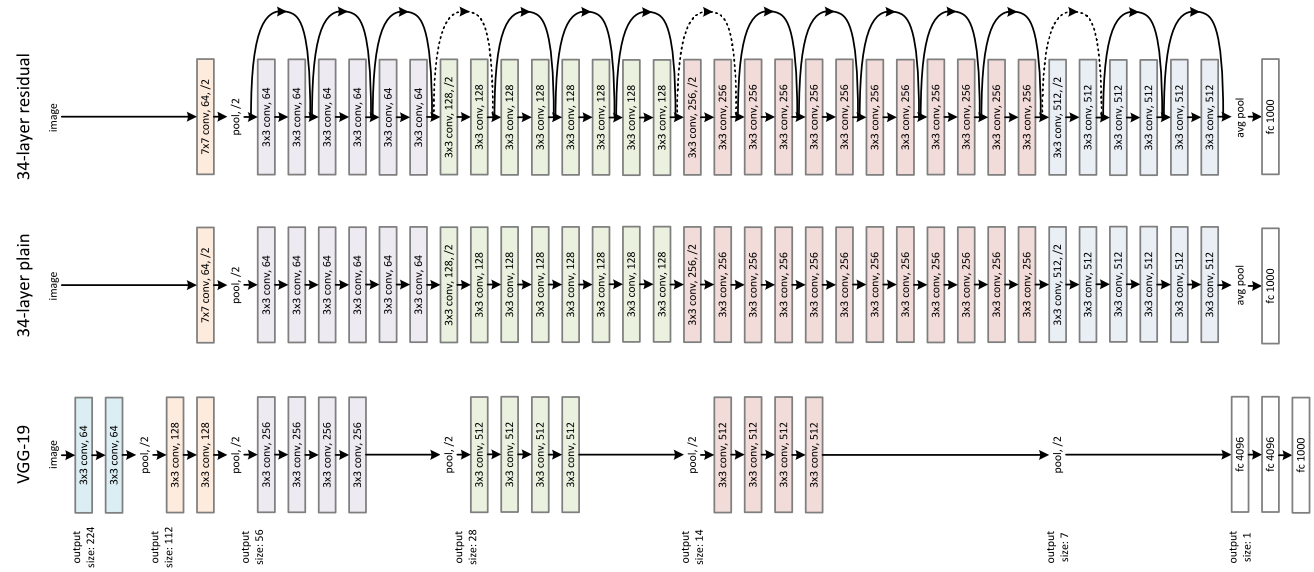
\includegraphics[scale=0.2]{img/ResNet.png}
	\caption{Perbandingan layer ResNet, plain, dan VGG-19 \cite{cit:10}}
	\label{fig:Resnet}
\end{figure}

\section{Pytorch}
\vspace{1ex}

\textit{Pytorch} merupakan sebuah library \textit{deep learning} pada \textit{Python} untuk menggantikan \textit{NumPy} dikarenakan membutuhkan kekuatan komputasi milik \textit{Graphics Processing Unit} (GPU). \textit{Library Pytorch} menyediakan fleksibilitas dan kecepatan komputasi maksimal ketika melakukan penelitian \textit{deep learning}. \textit{Pytorch} menyediakan \textit{pre-trained weights} dari model yang digunakan untuk mengklasifikasikan permasalahan lain sehingga dapat digunakan untuk mengurangi waktu dan kekuatan komputasi yang dibutuhkan. \cite{cit:11}
\vspace{1ex}

\section{\textit{Triplet Loss}}
\vspace{1ex}

\par \textit{Triplet Loss} merupakan sebuah \textit{Loss Function} yang umumnya digunakan dalam proses Re-Identifikasi. Pada fungsi ini dilakukan perbandingan jarak antara titik acuan terhadap titik positif yang merupakan gambar dalam kelas sama, dan perbandingan dengan titik negatif yang berasal dari kelas berbeda. Fungsi ini memastikan bahwa jarak ke titik positif akan lebih dekat dibandingkan dengan titik negatif.

\begin{figure}[h!]
	\centering
	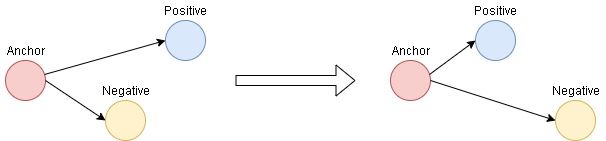
\includegraphics[scale=0.4]{img/TripletLoss.png}
	\caption{Triplet Loss}
	\label{fig:Triplet}
\end{figure}

\section{CycleGAN}
\vspace{1ex}

\begin{figure}  [!htb]
	        \captionsetup{justification=centering}
	        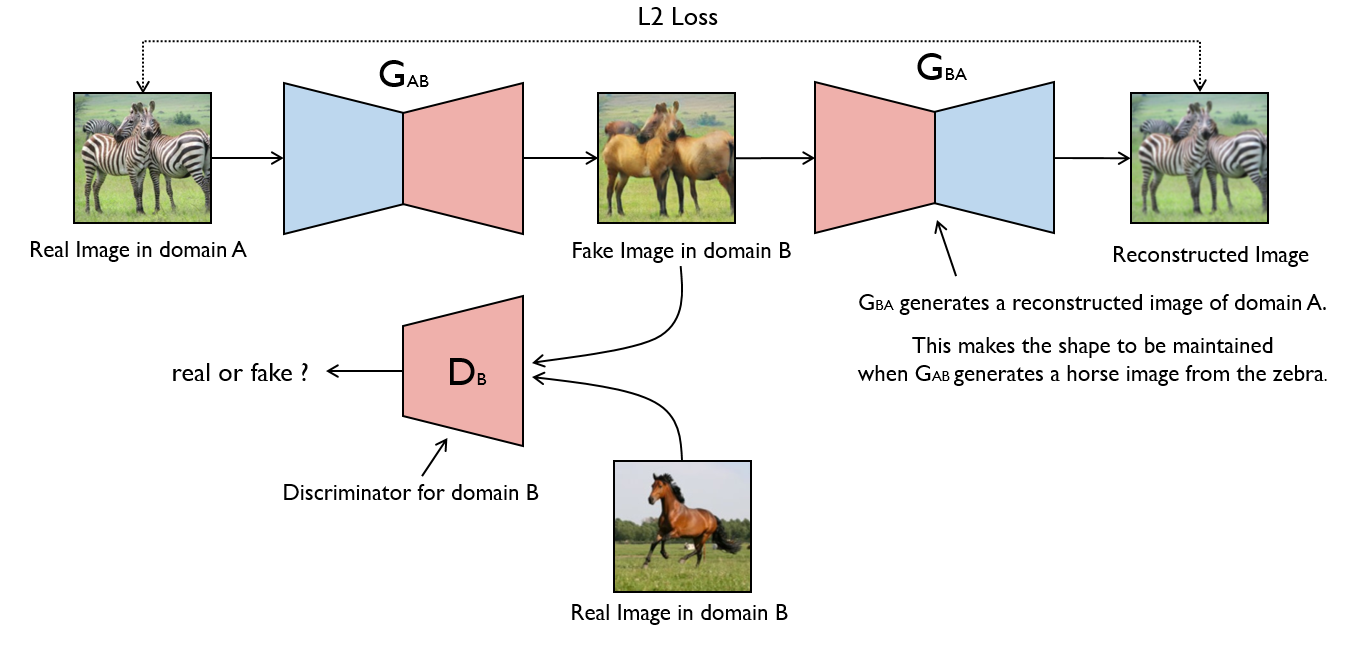
\includegraphics[scale=0.2]{img/cyclegan.png}
	        \caption{CycleGAN}
	        \label{fig: 3_18}
\end{figure}

CycleGAN merupakan sebuah teknik yang menggunakan \textit{Deep Convolutional Neural Network} untuk melakukan sinstesis sebuah gambar versi baru dengan modifikasi yang diinginkan, seperti mengubah gambar dari musim panas ke musim salju. Pada umumnya \textit{training} model untuk melakukan hal tersebut membutuhkan dataset dengan contoh berpasangan(\textit{paired example}) yang sangat besar. Cara seperti ini membutuhkan waktu yang sangat lama, dan pada beberapa kasus tertentu tidak dapat dilakukan. Namun dengan menggunakan CycleGAN, model dapat secara otomatis melakukan \textit{training} untuk translasi \textit{Image-to-image}.  dilatih secara \textit{unsupervised} dengan menggunakan kumpulan gambar dari sebuah domain X ke sebuah domain Y, tanpa harus memasangkan kedua gambar tersebut.

\section{\textit{Local Binary Pattern}}
\vspace{1ex}

\begin{figure}  [!htb]
	        \captionsetup{justification=centering}
	        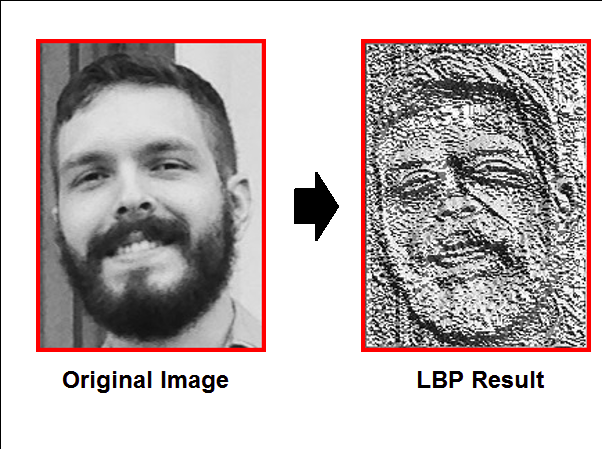
\includegraphics[scale=0.2]{img/lbp.png}
        	%\caption{Diagram alur kerja}
        	\caption{Local Binary Pattern}
        	\label{fig: 3_27}
\end{figure}

\textit{Local Binary Pattern} (LBP) merupakan salah satu deskriptor visual yang digunakan pada visi komputer. Pada umumnya LBP digunakan pada Face Recognition dikarenakan LBP merupakan deskriptor yang sangat kuat untuk melakukan klasifikasi tekstur. Selain itu telah ditemukan bahwa ketika LBP digabungkan dengan deskriptor \textit{Histogram of Oriented Gradients} (HOG), performa yang didapatkan bertambah secara drastis pada beberapa dataset tertentu.

\par Cara kerja dari LBP sendiri adalah sebagai berikut:
\begin{enumerate}
	\vspace{-2mm}
	\item Ubah citra menjadi bentuk \textit{grayscale} / hitam putih.
	\vspace{-2mm}
	\item Bagi citra menjadi beberapa bagian(\textit{cell})
	\vspace{-2mm}
	\item Untuk setiap \textit{pixel} yang terdapat pada sebuah \textit{cell}, bandingkan dengan pixel milik 8 neighbor yang terdapat di sekelilingnya
	\vspace{-2mm}
	\item Apabila nilai dari pixel yang di tengah lebih besar dari setiap pixel pada neighbornya maka pixel tersebut diberi nilai 0, selain itu pixel tersebut diberi nilai 1.
	\vspace{-2mm}
	\item Hitung Histogram
	\vspace{-2mm}
	\item Normalisasi Histogram.
\end{enumerate}

\cleardoublepage
\chapter{DESAIN DAN IMPLEMENTASI SISTEM}
\vspace{1ex}

\section*{}
	Penelitian ini dilaksanakan sesuai dengan desain sistem berikut dengan implementasinya. Desain sistem merupakan konsep dari pembuatan dan perancangan infrastruktur kemudian diwujudkan dalam bentuk blok-blok alur yang harus dikerjakan. Pada bagian implementasi merupakan pelaksanaan teknis untuk setiap blok pada desain sistem.
\vspace{1ex}

\section{Cakupan Tugas Akhir}
\vspace{1ex}

	Tugas akhir ini merupakan salah satu bentuk implementasi visi komputer untuk melakukan pencarian seorang individu dengan menggunakan gambar multi-modal, berikut pada Gambar 3.1 adalah cakupan Tugas Akhir dari Desain Sistem.
\begin{figure}  [!htb]
	\captionsetup{justification=centering}
	\includegraphics[scale=0.55]{img/Metodologi.png}
	\caption{Metodologi}
	\label{fig: 3_1}
\end{figure}
\vspace{1ex}
    \subsection{Penyesuaian Dataset}
    Desain sistem secara umum pada gambar \ref{fig: 3_1}, yang mencakup beberapa hal, salah satunya ialah penyesuaian dataset. Dataset PKU Sketch \cite{cit:15} Re-id yang digunakan akan melalui proses persiapan terlebih dahulu supaya dapat dilakukan training pada model. Penyesuaian yang akan dilakukan pada dataset meliputi, pemisahan dataset ke training dan testing, dan preprocessing seperti random horizontal flip, random erasing, dan lain sebagainya untuk meningkatkan presisi dari model sendiri. Selain itu pada dataset akan dibuat beberapa variasi untuk melakukan training dan testing, diantaranya adalah untuk melakukan pemrosesan dengan menggunakan CycleGAN pada gambar query sehingga terjadi translasi gaya pada gambar real ke gambar sketsa. 
    
	\subsection{Pembuatan Model}
	Setelah penyesuaian dataset telah dilakukan, pembuatan model ensemble akan dibuat dengan menggunakan Residual Network dengan pre-trained weights yang pernah digunakan untuk memecahkan masalah klasifikasi CIFAR, pada model ini fully connected layer yang terakhir akan dihapus dan diganti dengan dua fully connected layer baru. Pada fully connected layer baru yang pertama akan dilakukan pengenalan deskriptor masing masing individu, dan pada fully connected layer kedua akan dilakukan klasifikasi masing masing individu.

	\subsection{\textit{Training}}
	\textit{Training} pada dataset akan dilakukan setelah model telah dibuat. Training pada dataset PKU Sketch Re-id akan dilakukan menggunakan beberapa percobaan campuran untuk mencari model dengan efektivitas paling tinggi.
	
	\subsection{\textit{Testing}}
	\textit{Testing} akan dilakukan setelah training data telah berakhir, jika akurasi testing masih belum sesuai dengan harapan training akan dilakukan kembali. Evaluasi dari hasil test adalah menggunakan cara yang sama dengan yang terdapat pada paper milik Peking University\cite{cit:12}, dimana setiap metode dan variasi yang akan digunakan akan dinilai menggunakan rank-1 accuracy.
	
\pagebreak


\section{Desain Sistem}
\vspace{1ex}
	Pada Tugas Akhir ini, dilakukan penggabungan perangkat lunak berupa \textit{game engine} untuk mensimulasikan proses berkendara, dengan perangkat keras berupa \textit{controller} dari \textit{simulator} dan \textit{Microcontroller} untuk proses pengambilan data. Proses kerja dari sistem ini akan dijelaskan melalui diagram alur pada gambar \ref{fig: 3_2}.
	Selain itu, simulator ini memiliki 2 jenis data yang dapat diukur. Berikut penjelasan 2 macam jenis data tersebut.
\begin{figure}  [!htb]
	\captionsetup{justification=centering}
	\includegraphics[scale=0.25]{img/desainsistem.PNG}
	%\caption{Diagram alur kerja}
	\caption{Desain umum modul Simulator}
	\label{fig: 3_2}
\end{figure}
\vspace{1ex}

    \subsection{Data - Data Internal Simulator}
    \vspace{1ex}
    Jenis data yang pertama adalah data yang berasal dari dalam modul simulator, yaitu data - data seperti kecepatan mobil, informasi spasial seperti, sudut \textit{euler} \textit{(pitch,yaw,roll)} dan jarak relatif terhadap pinggir jalan, informasi tabrakan / \textit{colission}, serta informasi waktu respon / \textit{response time}. Data - data ini, disebut sebagai data internal, dikarenakan data - data tersebut bisa di ekstraksi langsung dari \textit{game engine}.
    
        \subsubsection{Kecepatan Mobil / \textit{Velocity}}
        
        Pada unity game engine, menggunakan library Unity. Bisa didapatkan secara langsung variabel - variabel yang berhubungan dengan kecepatan. Pada tugas akhir ini, dibutuhkan data kecepatan mobil relatif terhadap dunia atau biasa disebut \textit{global velocity}. Namun selanjutnya, data kecepatan global pun bisa dibagi menjadi 4 macam, yaitu : \textit{velocity} atau kecepatan kearah sumbu \textit{x}, \textit{velocity} atau kecepatan kearah sumbu \textit{y}, serta \textit{velocity} atau kecepatan kearah sumbu \textit{z}, ketiga hal tersebut bisa juga disebut kecepatan vektor \textit{x,y,z}. Dan yang terakhir, adalah \textit{velocity magnitude}, atau tingkat kebesaran suatu kecepatan berupa skalar. Contoh data ini bisa dilihat pada tabel pengujian \ref{tb:4_2}
        
        \subsubsection{Informasi Spasial}
        
        \begin{figure}  [!htb]
	        \captionsetup{justification=centering}
	        \includegraphics[scale=0.5]{img/relative-dist.jpg}
	        \caption{\textit{Relative Distance} \\ Oranye : Jarak dari \textit{Center of Mass} Mobil ke Batas Pinggir Kanan Jalan \\ Merah : Jarak dari \textit{Center of Mass} Mobil ke Batas Pinggir Kiri Jalan}
	        \label{fig: 3_19}
        \end{figure}
        
        Selain kecepatan, bisa didapatkan pula informasi spasial yang ada pada simulator. Pada tugas akhir ini, informasi spasial simulator adalah sudut euler yang merepresentasikan 6 derajat kebebasan atau biasa disebut \textit{6 Degree of Freedom (DoF))}, yaitu \textit{pitch, yaw,} dan \textit{roll} (gambar \ref{fig: 3_18}). Pada Tugas akhir ini, ketiga macam rotasi atau derajat kebebasan seluruhnya dimanfaatkan pada proses pembuatan desain jalan.
        
        \par Selanjutnya data spasial yang bisa didapatkan ialah posisi relatif kendaraan terhadap pinggir jalan (gambar \ref{fig: 3_19}). Dengan mengukur jarak terdekat dari titik pusat masa atau \textit{Center of Mass} mobil, ke batas pinggir kanan dan batas pinggir kiri jalan, dapat diketahui dimana posisi mobil di suatu lajur tersebut.
        
        \par Dengan menggabungkan dua macam jenis data tersebut, bisa didapatkan informasi yang sangat jelas tentang posisi dan orientasi dari kendaraan pengujian simulator ini. Yang nanti kedepannya sangat dibutuhkan untuk proses riset selanjutnya, yang akan memanfaatkan data - data tersebut.
        
        \subsubsection{Response Time}
        
        \begin{figure}  [!htb]
	        \captionsetup{justification=centering}
	        \includegraphics[scale=0.5]{img/jalur-tnp-mobil.JPG}
	        \caption{Response Time - IlustrasiJalur yang diharapkan - Kasus Tidak ada Mobil Lain}
	        \label{fig: 3_20}
        \end{figure}
        
        \begin{figure}  [!htb]
	        \captionsetup{justification=centering}
	        \includegraphics[scale=0.6]{img/jalur-dgn-mobil.JPG}
	        \caption{Response Time - Ilustrasi Jalur yang diharapkan - Kasus terdapat mobil lain}
	        \label{fig: 3_21}
        \end{figure}
        
        \textit{Response time} adalah metode pengukuran tingkat kewaspadaan pengemudi, dengan cara mendeteksi ketika pengemudi keluar dari lajur yang diharapkan. Lajur yang diharapkan disini, yang dimaksud ialah lajur sebelah kiri, dikarenakan desain simulator menggunakan model jalan yang ada di Indonesia. Berikut penjelasan tentang data \textit{Response time} pada gambar \ref{fig: 3_20} dan \ref{fig: 3_21}.
        
        Pada gambar \ref{fig: 3_20}, adalah gambar ilustrasi jalur yang diharapkan, pada kasus dimana tidak ada mobil lain didekat mobil pengujian. Warna hijau menandakan area yang di tandai oleh sistem simulator sebagai jalur yang diharapkan oleh sistem, artinya sistem mendeteksi bahwa mobil pada jalur yang telah sesuai serta pengemudi masih dalam keadaan waspada serta memiliki kontrol terhadap mobil. Apabila sistem mendeteksi mobil memasuki area yang berwarna merah, maka sistem akan melakukan pencatatan data yaitu kapan mobil mulai keluar dari jalur (tanggal dan waktu). Selanjutnya, sistem juga akan melacak mobil apabila mobil telah kembali ke area hijau, yang mana pada saat ini, sistem akan melakukan pencatatan data seberapa lama mobil telah keluar dari area hijau dengan \textit{unit} sekon, yang selanjutnya bisa didapatkan pula, seberapa lama mobil telah keluar dari area hijau dalam \textit{unit} hitungan \textit{frame}, dengan cara mengalikan waktu dalam sekon, dengan \textit{average framerate} dari simulator saat itu.
        
        \par Selanjutnya, pada gambar \ref{fig: 3_21}, adalah ilustrasi kasus dimana terdapat mobil didekat mobil uji, yang menyebabkan berubahnya jalur yang diharapkan. Apabila sistem mendeteksi terdapat mobil lain didekat mobil uji, sistem akan melakukan perubahan jalur yang diharapkan oleh sistem, metode penerapan pendeteksian seperti ini dapat diterapkan dengan banyak cara, salah satunya bisa dilakukan dengan membuat \textit{trigger box colission} disekitar mobil uji, yang mana ukurannya lebih besar dari \textit{bounding box} / ukuran mobil uji. Apabila terdapat suatu objek (seperti mobil lain), yang memasuki \textit{trigger box colission} dari mobil uji, maka bisa dilakukan perubahan pendeteksian jalur. Pada Tugas Akhir ini, digunakan metode ini untuk mendeteksi adanya mobil lain disekitar mobil uji, serta mendeteksi perlu terjadinya perubahan jalur yang diharapkan.
        
        \par Cara lain yang lebih mudah, namun tentunya dengan mengorbankan tingkat keakurasian pendeteksian yaitu adalah, dengan mengukur jarak mobil uji dengan mobil lain. Apabila jarak mobil uji dengan mobil lain ini dibawah nilai threshold, maka bisa dilakukan perubahan jalur yang diharapkan.
        
        \par Selanjutnya perlu digaris bawahi, bahwa sistem deteksi perubahan jalur ini juga sangat berkaitan dengan sistem deteksi terjadinya tabrakan. Sistem pendeteksian dan pencatatan data atau \textit{logging} dari \textit{colission event} ini akan dijelaskan pada subsubbab selanjutnya.
        
        \subsubsection{\textit{Colission Event}}
        
        \begin{figure}  [!htb]
	        \captionsetup{justification=centering}
	        \includegraphics[scale=0.65]{img/colliders.JPG}
	        \caption{2 Macam \textit{Colliders} Mobil - \textit{Box Collider} dan \textit{Mesh Collider}}
	        \label{fig: 3_22}
        \end{figure}
        
        \begin{figure}  [!htb]
	        \captionsetup{justification=centering}
	        \includegraphics[scale=0.7]{img/boundary-inside.JPG}
	        \caption{\textit{Boundary} dalam sirkuit}
	        \label{fig: 3_23}
        \end{figure}
        
        \begin{figure}  [!htb]
	        \captionsetup{justification=centering}
	        \includegraphics[scale=0.7]{img/boundary-outside.JPG}
	        \caption{\textit{Boundary} luar sirkuit}
	        \label{fig: 3_24}
        \end{figure}
        
         Pada subsubbab sebelumnya telah dijelaskan metode untuk mendeteksi keberadaan mobil lain di dekat mobil uji pada tugas akhir ini, yaitu dengan cara menggunakan \textit{trigger box event}. Pada subsubbab ini, \textit{colission event} yang dimaksud terdapat 2 macam. Yaitu yang pertama adalah, kejadian tabrakan dengan mobil lain, yang kedua kejadian tabrakan dengan pinggir jalan / \textit{boundary}. 
         
         \par Untuk proses pendeteksian tabrakan dengan mobil lain, dapat menggunakan \textit{mesh collider} yang sudah tersedia dengan mobil, untuk mempermudah proses deteksi, serta menyederhanakan \textit{physics interaction} antar mobil. Selain mobil uji, seluruh \textit{mesh collider} dari mobil lain ditentukan sebagai \textit{trigger}. Hal ini untuk menghindari terjadinya interaksi - interaksi yang tidak diinginkan ketika terjadi tabrakan antar mobil. 
         
         \par Dengan menggunakan fungsi \texttt{void onColissionEnter()} dan fungsi \texttt{void onTriggerEnter()} pada unity, dapat dilakukan pengecekan apabila terjadi overlap antar 2 \textit{GameObject} yang ada pada unity. Dengan menentukan \textit{GameObject} mana yang perlu dideteksi, sehingga langkah selanjutnya ialah mencatat data colission kedalam \textit{log file system}, 3 \textit{GameObject} yang perlu dideteksi adalah : \textit{Boundary} Luar / Batas Pinggir Kanan Jalan, \textit{Boundary} Dalam / Batas Pinggir Kiri Jalan, serta Mobil lain.
         
         \par Contoh data yang diambil pada \textit{colission event} bisa dilihat pada tabel \ref{tb:4_5}.
        
    
    \subsection{Data - Data Eksternal Simulator}
    \vspace{1ex}
    
     Selanjutnya Jenis data yang kedua adalah data yang berasal dari luar modul simulator, yaitu data - data seperti sinyal \textit{Electroencephalography (EEG)} / detak jantung pengemudi, dan atau data sinyal \textit{Electrooculography (EOG)} / data kedipan mata dari pengemudi, serta data citra wajah pengemudi menggunakan kamera. Data - data tersebut diatas, dikatakan sebagai data eksternal dikarenakan data - data tersebut didapatkan dari peralatan \textit{peripheral} yang dipasang pada modul simulator. Berhubung data EEG dan EOG merupakan data sinyal analog, maka diperlukannya suatu \textit{Analog to Digital Converter} atau ADC, supaya data bisa di rekam dalam \textit{log file}.
     Tentunya, perlu diperhatikan juga sampling rate dari ADC ini, sehingga bisa relevan dan dapat disesuaikan dengan data - data yang lain.
     
        \subsubsection{\textit{Serial Communication} Melalui \textit{port} COM}
        Pada tugas akhir ini, \textit{serial communication} melalui \textit{port} COM, dilakukan menggunakan \textit{Python}. Diagram \textit{flow chart} dari proses komunikasi data serial arduino ke PC, bisa di lihat pada gambar \ref{fig: 3_25}.
        \par Proses dari modul pembacaan data serial dimulai dengan pembuatan \textit{file} dengan nama tanggal dijalankannya modul tersebut. Hal ini dilakukan untuk mengetahui kapan waktu dan tanggal modul pembacaan dijalankan. Selain itu, hal ini memastikan bahwasanya file - file dapat dipisahkan atau disortir berdasarkan waktu dan tanggal, yang artinya data - data yang dicatat, tidak akan bercampur aduk dengan data - data percobaan yang sebelumnya.
        \par Dengan mengasumsikan bahwa arduino akan melakukan pengiriman data, \textit{python} akan terus membaca data dari arduino, dengan maksimum \textit{baudrate} yang telah ditentukan. Kemudian, setelah proses pembacaan dilakukan, akan dilakukan proses \textit{decode}. Proses \textit{Decode} ialah proses dimana \textit{python} akan melakukan konversi data biner, menjadi data - data diskrit \textit{integer} / bilangan bulat, yang kemudian hasil dari proses \textit{decode}, akan dilakukan proses append pada \textit{file} yang telah dibuat sebelumnya. 
        \par Informasi lebih jelas tentang proses \textit{append file} dan \textit{log file system} akan dijelaskan lebih lanjut pada sub-bab \ref{logfilesystem}
        
        \subsubsection{Citra Wajah Pengemudi / \textit{Webcam}}
        Pada \textit{Unity Game Engine}, sistem mensupport pembacaan informasi kamera webcam sebagai salah satu bagian dari \textit{library mobile camera information}, yang artinya adalah, apabila platform dari simulator menggunakan PC dengan OS \textit{Windows}, dan terdapat \textit{peripheral Webcam} yang terpasang, Unity dapat mendeteksi \textit{webcam} tersebut sebagai \textit{Imaging Device}.
        \par Sebagai \textit{Imaging Device}, data yang diperoleh unity dari \textit{webcam} ditangkap sebagai \textit{texture information}, atau informasi texture dari suatu \textit{GameObject}.
        
        \begin{figure}  [!htb]
	        \captionsetup{justification=centering}
	        \includegraphics[scale=0.62]{img/webcam-texture.JPG}
	        \caption{Kubus yang memiliki \textit{texture information} dari \textit{Webcam / Imaging Device}}
	        \label{fig: 3_26}
        \end{figure}
        
       Dikarenakan informasi yang ditangkap oleh unity merupakan suatu \textit{texture}, maka \textit{texture} tersebut bisa di pasangkan ke suatu \textit{GameObject}, agar memiliki tampilan dari \textit{webcam}.  Bisa dilihat, pada gambar \ref{fig: 3_26}, ketika informasi webcam di pasangkan dengan kubus.
       \par Namun pada tugas akhir ini, yang dibutuhkan bukanlah informasi \textit{texture} yang bisa digunakan oleh game ini. Yang dibutuhkan adalah \textit{frame - frame} / gambar wajah dengan \textit{timestamp} yang sesuai. Maka langkah selanjutnya adalah mengekstrak informasi \textit{texture} tersebut keluar dari unity. Hal ini mudah dilakukan dengan melakukan fungsi \textit{encoding} ke tipe \textit{file} yang berekstensi \textit{PNG}. Setelah encoding dilakukan, \textit{file stream} akan menuliskan data hasil \textit{encoding} menjadi suatu gambar lengkap dengan \textit{timestamp} nya.
       \par Hasil pengujian pengambilan data citra wajah pengemudi menjadi frame - frame yang telah di \textit{encode} menjadi PNG bisa di lihat pada gambar \ref{fig:4.2}
    
\section{Desain Lajur Simulator}
\vspace{1ex}

    \par Pada tugas akhir ini, terdapat 4 macam lajur yang dapat dipilih oleh pengemudi. 4 Macam lajur tersebut berfungsi sebagai basis riset untuk mengeliminasi terjadinya bias atau pengaruh yang dihasilkan oleh perbedaan jumlah lajur yang digunakan.
    
\begin{figure}  [!htb]
	\captionsetup{justification=centering}
	\includegraphics[scale=0.31]{img/2lj_short_oh.jpg}
	\caption{Desain sirkuit 2 lajur dengan jarak yang pendek dan kompleksitas yang rendah}
	\label{fig: 3_3}
\end{figure}
\vspace{1ex}

\begin{figure}  [!htb]
	\captionsetup{justification=centering}
	\includegraphics[scale=0.53]{img/2lj_long_oh.jpg}
	\caption{Desain sirkuit 2 lajur dengan jarak yang panjang dan kompleksitas yang tinggi}
	\label{fig: 3_4}
\end{figure}
\vspace{1ex}

\begin{figure}  [!htb]
	\captionsetup{justification=centering}
	\includegraphics[scale=0.53]{img/3lj_oh.jpg}
	\caption{Desain sirkuit 3 lajur}
	\label{fig: 3_5}
\end{figure}
\vspace{1ex}

\begin{figure}  [!htb]
	\captionsetup{justification=centering}
	\includegraphics[scale=0.53]{img/4lj_oh.jpg}
	\caption{Desain sirkuit 4 lajur}
	\label{fig: 3_6}
\end{figure}
\vspace{1ex}

    \par Berikut pada Gambar \ref{fig: 3_3}, \ref{fig: 3_4}, \ref{fig: 3_5}, dan \ref{fig: 3_6}, adalah tampak atas dari desain - desain lajur yang digunakan pada simulator ini, seluruh lajur didesain dengan bentuk \textit{closed-loop circuit}. Hal ini bertujuan agar mengurangi ukuran aset jalan yang akan digunakan. Selain itu desain seperti ini dapat berdampak pada durasi pengambilan data, desain sirkuit yang \textit{closed-loop} memungkinkan kegiatan proses pengambilan data supaya tidak bergantung pada panjang jalan yang digunakan.
    \par Tabel \ref{tb:3_1} adalah detil informasi dari desain jalan / sirkuit yang dibuat pada simulator ini. 
    
\begin{table}[]
\caption{Tabel Informasi Sirkuit Jalan}
\label{tb:3_1}
\begin{tabular}{|c|c|c|c|c|c|}
\hline
\multirow{2}{*}{No.} & \multirow{2}{*}{\begin{tabular}[c]{@{}c@{}}Jumlah Lajur\\ (Unit)\end{tabular}} & \multirow{2}{*}{\begin{tabular}[c]{@{}c@{}}Jarak\\ (Unit)\end{tabular}} & \multirow{2}{*}{\begin{tabular}[c]{@{}c@{}}Lebar\\ (Unit)\end{tabular}} & \multicolumn{2}{c|}{\begin{tabular}[c]{@{}c@{}}Kompleksitas\\ (Tampak Atas)\end{tabular}} \\ \cline{5-6} 
                     &                                                                                &                                                                         &                                                                               & \textit{CW Curve}                           & \textit{CCW Curve}                          \\ \hline
1                    & 2                                                                              & 43,145                                                                  & 12                                                                            & 4                                           & 0                                           \\ \hline
2                    & 2                                                                              & 260.226                                                                 & 12                                                                            & 6                                           & 10                                          \\ \hline
3                    & 3                                                                              & \multicolumn{1}{l|}{260.226}                                            & 16                                                                            & 6                                           & 10                                          \\ \hline
4                    & 4                                                                              & 411.346                                                                 & 20                                                                            & 11                                          & 12                                          \\ \hline
\end{tabular}
\end{table}
    
\section{Desain \textit{Behaviour} dari Kendaraan Lain}
\vspace{1ex}

    \par Pada Tugas akhir ini, Desain dari \textit{AI Behavior} kendaraan lain cukup mengikuti lajur sirkuit sesuai dengan jalur yang telah didefinisikan oleh \textit{Bézier curve}, kemudian pada script \textit{follower} yang ada di unity, dikarenakan desain lajur yang \textit{closed-loop}, perlu di definisikan arah dari kendaraan tersebut, dilihat dari tampak atas, apakah kendaraan memiliki \textit{clockwise path} atau \textit{counter-clockwise path}.
    \par Selain arah dari kendaraan, diperlukannya pendefinisian kecepatan kendaraan tersebut, pada Tugas Akhir ini kecepatan kendaraan ditentukan dengan randomisasi dalam suatu rentang tiap kali simulator dijalankan.
    \par Informasi detil dari desain AI kendaraan lain di \textit{unity}, dapat dilihat pada tabel \ref{tb:3_2}

\begin{table}[]
\caption{Tabel Informasi AI Tiap - Tiap Tipe Lajur}
\label{tb:3_2}
\begin{tabular}{|c|c|c|c|c|c|c|}
\hline
\multirow{2}{*}{No.} & \multirow{2}{*}{Lajur} & \multirow{2}{*}{\begin{tabular}[c]{@{}c@{}}Jumlah\\ Mobil\end{tabular}} & \multicolumn{2}{c|}{\textit{AI Rotation}}             & \multicolumn{2}{c|}{\textit{\begin{tabular}[c]{@{}c@{}}Velocity\\ (Unit/Frame)\end{tabular}}} \\ \cline{4-7} 
                     &                        &                                                                         & \textit{CW}               & \textit{CCW}              & \textit{Min}                                  & \textit{Max}                                  \\ \hline
1                    & \textit{2 (Short)}     & 1                                                                       & \xmark     & \checkmark & 5.0f                                          & 15.0f                                         \\ \hline
2                    & \textit{2 (Long)}      & 2                                                                       & \checkmark & \checkmark & 0.1f                                          & 0.9f                                          \\ \hline
3                    & 3                      & 3                                                                       & \checkmark & \checkmark & 0.1f                                          & 0.9f                                          \\ \hline
4                    & 4                      & 4                                                                       & \checkmark & \checkmark & 0.01f                                         & 0.1f                                          \\ \hline
\end{tabular}
\end{table}

\section{Alur Kerja}
\vspace{1ex}

Pembuatan tugas akhir ini dibagi menjadi beberapa tahapan, yaitu:
    \begin{enumerate}[nolistsep]
	
	\item \nohyphens{Pembuatan Simulasi Menggunakan \textit{Unity Game Engine}}
	\item Pengaturan dan Konfigurasi \textit{Steering Wheel Controller} 
	\item Pembuatan Modul Pengambilan Data dengan \textit{Microcontroller}
	\item Penggabungan Seluruh Sistem Menjadi Satu Modul
	
	\end{enumerate}

\section{Pembuatan Simulasi Menggunakan \textit{Unity Game Engine}}
\vspace{1ex}
   Pada Tugas Akhir ini, proses pembuatan simulasi menggunakan \textit{Unity Game Engine}. Namun tidak hanya menggunakan \textit{Unity Game Engine} saja, tentunya selain memanfaatkan \textit{unity editor}, juga diperlukan \textit{source code editor}, pada tugas akhir ini menggunakan \textit{Visual Studio 2017}. Selain itu terdapat \textit{tools - tools} lain di luar \textit{unity} yang dapat mempermudah proses pembuatan Simulator ini.
	
	\subsection{Pembuatan Sirkuit Jalan}
	\vspace{1ex}
	
	\begin{figure} [!htb]
	    \captionsetup{justification=centering}
	    \includegraphics[scale=0.25]{img/shanghai-ic.png}
	    \caption{\textit{Shanghai International Circuit\cite{cit:14}}}
	    \label{fig: 3_10}
    \end{figure}
	
	\begin{figure} [!htb]
	    \captionsetup{justification=centering}
	    \includegraphics[scale=0.36]{img/bezier-curve-jalan.JPG}
	    \caption{5 Macam \textit{Bézier curve} sirkuit (dari kiri ke kanan) : batas kiri jalan, \textit{Vehicle AI Path - Counterclock Wise}, tengah lajur / marka jalan, \textit{Vehicle AI Path - Clock Wise}, serta batas kanan jalan }
	    \label{fig: 3_9}
    \end{figure}
	
	Proses pembuatan sirkuit jalan adalah proses yang paling memakan waktu pada tugas akhir ini. Yang pertama perlu dilakukan adalah mendefinisikan \textit{path} jalan menggunakan \textit{Bézier curve}, atau jalur yang akan digunakan sebagai \textit{base} dari \textit{3d mesh} jalan atau lajur itu sendiri, salah satu contohnya adalah pada gambar \ref{fig: 3_9}, bisa dilihat terdapat 5 macam kurva bezier yang dapat ditemukan. Semua 5 kurva tersebut dibutuhkan untuk proses kalkulasi informasi jarak serta informasi \textit{colission} yang nantinya akan disimpan kedalam \textit{log file}.
	\par Menggunakan \textit{Shanghai International Circuit} dari \textit{Formula 1}, sebagai referensi bentuk dari sirkuit, diperlukannya penyesuaian tingkat kelengkungan dari belokan yang ada pada sirkuit referensi. Untuk menghindari \textit{mesh overlap}, maka tiap - tiap tikungan yang tajam, perlu diperhalus sedemikian hingga \textit{mesh overlap} agar tidak terjadi. Namun tidak terlalu dikurangi sehingga pengemudi tetap waspada terhadap tikungan tersebut, serta supaya pengemudi mengurangi kecepatan sebelum melakukan belokan tersebut.
	\par Hal ini penting, dikarenakan pada saat proses pengujian berjalan, mobil tidak diharapkan untuk keluar dari lajur pengujian.
	    
	    \subsubsection{\textit{Editing Tools : Path Creator}}
	    \vspace{1ex}
	    
	    \begin{figure} [!htb]
	        \captionsetup{justification=centering}
	        \includegraphics[scale=0.47]{img/bezier-curve-cp.JPG}
	        \caption{\textit{Bézier curve} tampak atas, merah : \textit{anchor points}, biru : \textit{control points}}
	        \label{fig: 3_11}
        \end{figure}
        
        \begin{figure} [!htb]
	        \captionsetup{justification=centering}
	        \includegraphics[scale=0.35]{img/bezier-curve-cp2.JPG}
	        \caption{\textit{Bézier curve} pada \textit{3d plane}}
	        \label{fig: 3_12}
        \end{figure}
	    
	    Untuk memudahkan proses pembuatan \textit{Bézier curve}, pada unity. Penulis menggunakan \textit{tools} yang tersedia di unity yang berfungsi untuk mempermudah kalkulasi matematis serta proses \textit{scripting} yang ada pada unity untuk menghasilkan kurva tersebut. Tools tersebut ialah \textit{Path Creator} oleh Sebastian Lague, Path Creator ini dipilih dikarenakan, memudahkan dalam proses manipulasi kurva \textit{Bézier}. Dikarenakan pada \textit{unity} tidak mensupport kurva \textit{Bézier} secara natif, maka biasanya para \textit{game developer}, membuat \textit{script} mereka masing - masing untuk membuat kurva \textit{Bézier}, dengan melakukan kalkulasi persamaan matematis pada script mereka tersebut, kemudian diperlukannya manipulasi titik - titik kontrol sesuai dengan \textit{script} tersebut.
	    \par Namun \textit{Path Creator} memungkinkan penulis untuk melewati proses kalkulasi matematis serta pendefinisian titik - titik kontrol, langsung ke proses manipulasi \textit{drag and drop} titik - titik kontrol, pada \textit{Unity Editor}.
	    \par Pada gambar \ref{fig: 3_11} dan \ref{fig: 3_12}, bisa dilihat titik - titik yang dapat dimanipulasi menggunakan \textit{Path Creator}. Warna merah menunjukkan \textit{anchor points}, yang artinya titik tersebut merupakan titik - titik statis pada suatu persamaan kurva, dengan memanipulasi lokasi dari \textit{anchor points} pada 3 dimensi, dapat didapatkan bentuk \textit{approximation} dari target sirkuit diinginkan. Tentunya, semakin banyak \textit{anchor points} yang digunakan, semakin akurat pula \textit{approximation} jalan yang dibuat. Namun tentunya, kurva jalan menjadi lebih kompleks serta lebih sulit untuk dimanipulasi.
	    \par Kemudian, warna biru menunjukkan \textit{control points}, \textit{control points} ini menentukan lengkungan yang diharapkan diantara tiap - tiap \textit{anchor points}, tentunya agar didapatkankannya lengkungan yang sesuai dengan belokan yang ada pada sirkuit referensi, titik - titik inilah yang akan dapat dimanipulasi.
	    
	    \subsubsection{\textit{Plane Projection} serta \textit{Normal Vector}}
        
        Pada Tugas Akhir ini, informasi tentang \textit{plane projection} yang ada pada kurva \textit{Bézier} sangat penting. Hal ini dapat menunjukkan informasi tentang kekasaran medan atau \textit{level} ketinggian dari suatu daerah pada \textit{terrain} yang ada pada jalan.
        
        \par Pada Tugas akhir ini, jalan yang memiliki 2 dan 3 lajur, memiliki \textit{plane projection} terhadap \textit{XZ Plane}, artinya medan yang ada pada kedua macam jumlah lajur tersebut memiliki kedataran yang seragam, tidak memiliki tanjakan ataupun turunan. 
        
        \par Sedangkan, pada jalan yang memiliki 4 lajur, dengan memanfaatkan semua sumbu \textit{XYZ} maka dapat dihasilkan jalur yang memiliki tanjakan dan turunan.
        
        \begin{figure} [!htb]
	        \captionsetup{justification=centering}
	        \includegraphics[scale=0.35]{img/pp1.JPG}
	        \caption{\textit{Normal Force} Jalan (\textit{Yaw} 0 Derajat)}
	        \label{fig: 3_13}
        \end{figure}
        
        \begin{figure} [!htb]
	        \captionsetup{justification=centering}
	        \includegraphics[scale=0.35]{img/pp2.JPG}
	        \caption{\textit{Normal Force} Jalan (\textit{Yaw} 60 Derajat)}
	        \label{fig: 3_14}
        \end{figure}
        
        Kemudian selanjutnya adalah, penentuan \textit{normal force}. Pada \textit{path creator}, parameter yang dapat dikontrol adalah \textit{global angle}, dari normal force tersebut. Hal ini menentukan sudut rotasi / \textit{yaw}, dari jalan yang dibuat pada path yang ditentukan.
        \par Berikut pada gambar \ref{fig: 3_13} dan gambar \ref{fig: 3_14}, perbandingan efek dari \textit{normal force} yang ada di jalan. Hal ini penting diperhatikan untuk proses desain serta pembuatan jalan, yang memanfaatkan seluruh 6 derajat kebebasan \textit{(Degree of Freedom)}, \textit{pitch, yaw,} dan \textit{roll}
	
	\subsection{Pembuatan \textit{Terrain}}
	\vspace{1ex}
	
	Medan atau \textit{terrain}, merupakan kanvas kosong dari sebuah \textit{scene}, yang dapat diisi dengan berbagai macam objek - objek estetis untuk meningkatkan realisme dan imersivitas pada proses simulasi. Pada tugas akhir ini medan yang dibuat pada tiap lajur tidak terlalu berpengaruh terhadap proses pengambilan data itu tersendiri, namun merupakan salah satu \textit{design choice} atau proses pemilihan desain agar meningkatkan kualitas dari \textit{user experience}.
	
	\par Setelah proses pembuatan jalan selesai, untuk meningkatkan estetika, diperlukannya \textit{terrain} yang mengelilingi jalan. Pada \textit{Unity,} objek - objek \textit{non-colission} dapat ditaruh untuk meningkatkan estetika tersebut. Seperti contohnya, pohon - pohon dan semak - semak atau rerumputan. Selain itu, dapat diterapkan perubahan kontur dari \textit{terrain}. Seperti contohnya dapat diterapkan proses peninggian sebagian dari \textit{terrain} untuk menghasilkan bukit, atau bahkan sebaliknya, proses penurunan dari sebagian \textit{terrain} dapat menghasilkan lembah.
	
    Selain itu, pada \textit{unity} dapat ditambahkannya tekstur pada \textit{terrain}. Tekstur disini yang dimaksud ialah, warna atau gambar yang dapat diterapkan pada \textit{terrain} agar menghasilkan corak pada \textit{terrain}. Seperti contohnya tekstur dari tanah coklat, atau tekstur warna pasir kuning, dan sebagainya.
    
    \begin{figure} [!htb]
	    \captionsetup{justification=centering}
	    \includegraphics[scale=0.35]{img/terrain.JPG}
	    \caption{\textit{Terrain} setelah ditambahkan bukit, dan pepohonan}
	    \label{fig: 3_17}
    \end{figure}
    
    Selanjutnya, perlu di garis bawahi juga, pada Tugas Akhir ini, salah satu \textit{design choice} merupakan jalan berbentuk sirkuit, maka dari itu terrain, untuk mengakomodasi hal tersebut di terapkan bukit yang mengelilingi sirkuit jalan, untuk memberikan kesan bahwasanya mobil tidak dapat keluar dari lajur.
    
    \subsection{\textit{Menu} dan \textit{User Interface}}
    
    Proses pembuatan Menu dibutuhkan untuk memudahkan pemilihan jumlah lajur nanti setelah simulator menjalani proses \textit{build}. Menu disini dibutuhkan agar tidak terlalu kompleks, namun cukup agar menu dapat menjelaskan serta merepresentasikan tampilan atau tombol yang ditekan. Pemilihan yang intuitif serta fungsionalitas yang berjalan sudah cukup untuk proses ketika di menu.
    \par Perlu diperhatikan juga, dapat diterapkan pula \textit{asynchronous loading}, pada menu ini. Artinya, \textit{scene} atau jenis lajur yang dipilih, akan di muat sebelum tombol ditekan. Supaya proses \textit{loading} akan menjadi lebih cepat.
    
    \begin{figure} [!htb]
	    \captionsetup{justification=centering}
	    \includegraphics[scale=0.35]{img/menuUI.JPG}
	    \caption{\textit{User Interface} dari Menu}
	    \label{fig: 3_15}
    \end{figure}
    
    Gambar \ref{fig: 3_16} adalah, gambar yang menunjukkan hasil menu yang dibuat. Terdapat 4 tombol yang bisa ditekan, tiap - tiap tombol memiliki penjelasan \textit{text} yang jelas, yaitu merepresentasikan tombol yang akan membawa \textit{user} menuju \textit{scene} atau lajur yang sesuai dengan text tersebut, seperti 2 lajur pendek, 2 lajur panjang, 3 lajur, serta 4 lajur. Selain itu, dipasang pula \textit{background canvas} serta logo ITS pada \textit{User Interface} Menu.
    
    \subsection{\textit{Log File System} dan \textit{Kalkulasi Data}} 
    \label{logfilesystem}
    
    \textit{Log File System} adalah salah satu komponen penting dari Tugas Akhir ini, agar didapatkan suatu \textit{Log File System}, beberapa macam komponen dibutuhkan dari sistem ini (gambar \ref{fig: 3_15}).
    
    \begin{figure} [!htb]
	    \captionsetup{justification=centering}
	    \includegraphics[scale=0.5]{img/logfile.JPG}
	    \caption{Diagram \textit{Log File System}, proses ekstraksi data, dan proses \textit{append data}}
	    \label{fig: 3_31}
    \end{figure}
    
    Yang pertama adalah, proses ekstraksi data. Proses ini sangat mudah dikarenakan informasi - informasi yang dibutuhkan sudah tersedia dan tertulis pada variabel - variabel yang dipakai pada simulasi serta komunikasi \textit{serial data}. 
    \par Setelah proses ekstraksi data yang dibutuhkan, selanjutnya dibuatlah komunikasi \textit{file stream} dari \textit{unity} ke \textit{OS file system}, pada Tugas Akhir ini, OS yang digunakan adalah Windows 8.1. Komunikasi file stream yang dibuat bertugas untuk mengecek apakah \textit{path} dari direktori yang dituju sudah ada, apabila belum tersedia folder yang diharapkan, maka \textit{file stream}, akan membuat folder pada direktori yang diinginkan dan membuat \textit{file - file} sesuai dengan \textit{output data} yang ada.
    \par Langkah selanjutnya adalah \textit{file stream} akan membuka \textit{file} yang telah dibuat tersebut, kemudian melakukan \textit{append}, atau penambahan data kedalam \textit{file} tersebut. Jenis \textit{Append} yang pertama kali dilakukan adalah melakukan \textit{append header}, atau informasi - informasi pada ujung tabel (label), serta informasi \textit{separator} dari kolom. Pada Tugas Akhir ini, seluruh \textit{output file}, menggunakan \textit{separator} kolom berupa \textit{tab} atau simbol \textit{\textbackslash t} sedangkan separator baris berupa \textit{line break} atau simbol \textit{\textbackslash n}
    

\section{Pengaturan dan Konfigurasi \textit{Steering Wheel Controller}}
\label{steeringwheelconf}
\vspace{1ex}
    \begin{figure}  [!htb]
	    \captionsetup{justification=centering}
	    \includegraphics[scale=0.51]{img/steeringwheel.jpg}
	    %\caption{Diagram alur kerja}
	    \caption{Diagram Steering Wheel yang digunakan, \textit{Sumber : Buku Manual PXN Steering Wheel}}
	    \label{fig: 3_28}
    \end{figure}

	Konfigurasi kontroller yang perlu dilakukan adalah salah satunya melakukkan \textit{mapping} tombol - tombol dari keyboard ke tombol - tombol serta perangkat analog dari \textit{steering wheel controller} yang digunakan, seperti contohnya perangkat analog yang perlu dilakukan \textit{sampling} adalah pedal, \textit{sampling} yang dimaksud adalah melakukan pembagian data voltase analog yang ada di pedal menjadi nilai - nilai diskrit yang kemudian dapat dikonversikan ke kecepatan mobil, sesuai nilai - nilai diskrit yang didapatkan. Selain itu juga perlu dilakukan kalibrasi mode sudut dari steering wheel yang memiliki 2 macam mode, yaitu mode 270 derajat putaran, serta 900 derajat putaran. 
	Pada Tugas akhir ini, \textit{steering wheel} akan menggunakan mode 270 derajat, serta proses pergantian gigi \textit{(gear shift)} menggunakan proses manual tanpa kopling. Hal ini dikarenakan keterbatasan perangkat keras yang digunakan.
	
	\begin{figure}  [!htb]
	    \captionsetup{justification=centering}
	    \includegraphics[scale=0.3]{img/driverinput.JPG}
	    %\caption{Diagram alur kerja}
	    \caption{Grafik hasil \textit{plotting} data \textit{input} pengemudi}
	    \label{fig: 3_29}
    \end{figure}
    
    Berikut pada gambar \ref{fig: 3_28} adalah \textit{key map} dari sistem simulator tugas akhir ini. proses kalibrasi pedal gas dan rem disambungkan ke \textit{vertical axis / axis y} dari \textit{unity controller}, maka bisa didapatkan nilai dari pedal atau rem tersebut, berupa data \textit{float} yang memiliki rentang 0 hingga 1. Sedangkan kalibrasi \textit{steering wheel} disambungkan dengan \textit{horizontal axis / axis x} dari \textit{unity controller}, yang memiliki data berupa \textit{float} dengan rentang -1 hingga 1.
    \par Kemudian, data \textit{float} tersebut, dapat dilakukan proses kalkulasi untuk mendapatkan sudut dari pedal gas dan rem, serta sudut dari \textit{steering wheel}, sehingga dapat dilakukan proses \textit{plotting} seperti berikut pada gambar \ref{fig: 3_29}
    
    Selain \textit{vertical axis} dan \textit{horizontal axis}, terdapat pula tombol - tombol lain dari \textit{steering wheel controller} yang digunakan. Yaitu tombol \textbf{X} untuk menyalakan mesin dari mobil \textit{(starter)}, selain itu ada tombol \textit{R-Paddle} dan \textit{L-Paddle} untuk menaikkan dan menurunkan gigi mesin secara berurutan. Proses ini, tidak memerlukan kopling, cukup menekan tombol \textit{L-R-Paddle} untuk menaikkan atau menurunkan gigi mobil.
    
    \par Di tengah \textit{steering wheel} juga terdapat \textit{switch} untuk mengganti mode \textit{steering} yaitu mode 270 derajat atau 900 derajat.
\section{Pembuatan Modul Pengambilan Data dengan \textit{Microcontroller}}
\label{microcontroller}
\vspace{1ex}

    \begin{figure}  [!htb]
	    \captionsetup{justification=centering}
	    \includegraphics[scale=0.2]{img/sinyaldangambar.JPG}
	    %\caption{Diagram alur kerja}
	    \caption{Diagram Sinkronisasi \textit{capture rate} kamera dengan \textit{sampling rate} dari sensor arduino}
	    \label{fig: 3_30}
    \end{figure}
    
    Pembuatan modul pengambilan data serial seperti EEG dan ECG, dapat dilakukan menggunakan Arduino, sehingga perlu disiapkan port USB. Sedangkan pengambilan data berupa gambar wajah pengemudi menggunakan kamera, dapat disambungkan langsung ke \textit{Unity Game Engine} dan dapat langsung disimpan ke \textit{harddrive} komputer simulator. Hal ini dilakukan agar data yang masuk berupa gambar wajah pengemudi serta sinyal - sinyal yang di peroleh oleh \textit{microcontroller} dapat di lakukan pengolahan dan proses analisa.
    Perlu di perhatikan juga \textit{sampling rate} dari sistem pengambilan sinyal arduino, dengan \textit{capture rate} dari \textit{webcam}, kedua data tersebut perlu di sinkronkan dengan memperhatikan kedua nilai tersebut. \textit{Sampling rate} dari arduino disini bisa didapatkan dari \textit{datasheet} sensor yang digunakan, kemudian dilakukan kalkulasi dengan \textit{margin of error} yang disebabkan oleh kegagalan transmisi data dari arduino ke komputer simulator melalui kabel USB, agar didapatkan hasil yang dapat diterima. Sedangkan \textit{capture rate} dari kamera merupakan seberapa banyak gambar atau \textit{frame} yang diambil oleh kamera tiap \textit{frame} yang di proses oleh simulator. Pada Tugas Akhir ini, target capture rate adalah 1:1. Yang artinya, kamera akan mengambil gambar wajah pengemudi tiap frame game tersebut dijalankan. Berikut pada gambar \ref{fig: 3_30} adalah diagram dari penjelasan sinkronisasi kedua data tersebut, menjadi suatu modul analisis sinyal dengan gambar wajah.
    
\section{Penggabungan Seluruh Sistem Menjadi Satu Modul}
\vspace{1ex}
    Langkah terakhir adalah mengintegrasikan seluruh sistem menjadi satu modul yang utuh, supaya dapat melakukan pengolahan data dengan irisan waktu \textit{(t)} yang bersamaan. Keluaran yang diharapkan adalah, simulator dapat melakukan pengambilan data analog, data citra gambar, serta data - data internal simulasi secara bersamaan dan integrasi. Seperti yang dijelaskan pada bab \ref{logfilesystem} hingga bab \ref{steeringwheelconf}, Penggabungan Sub - sub modul, menjadi satu modul utuh adalah seperti berikut
    
    \begin{enumerate}[nolistsep]
	
	\item Sub-modul pengambilan data internal, mencakup :
	    \begin{enumerate}[nolistsep]
	        \item Sub-Modul Kecepatan Mobil
	            \begin{enumerate}
	                \item Kecepatan Vektor Sumbu \textit{x,y,z}
	                \item \textit{Magnitude} Kecepatan Vektor
	            \end{enumerate}
	        \item Sub-Modul Informasi Spasial
	            \begin{enumerate}
	                \item Posisi Relatif Mobil terhadap jalan
	                \item Sudut Euler dan \textit{6 Degree of Freedom} - Pitch, Yaw, Roll
	            \end{enumerate}
	        \item Sub-Modul Respon Pengemudi
	            \begin{enumerate}
	                \item Informasi Respon Pengemudi Ketika kendaraan keluar jalur
	                \item Informasi \textit{Input} dari Steering Wheel Controller (Sudut \textit{Steering Wheel} dan Nilai Tekanan Pedal Gas dan Rem)
	            \end{enumerate}
	    \end{enumerate}
	\item Sub-modul pengambilan data eksternal, mencakup :
	    \begin{enumerate}[nolistsep]
	        \item Sub-Modul Sinyal dan Citra Wajah
	            \begin{enumerate}
	                \item Sinyal dari sensor, bisa berupa ECG, EEG, atau EOG
	                \item Citra Wajah tiap frame dari kamera
	            \end{enumerate}
	    \end{enumerate}
	
	\end{enumerate}
    
Pada tugas akhir ini, sub - sub modul dibentuk berdasarkan kebutuhan proses pengujian, namun untuk riset kedepannya, proses pembuatan serta sinkronisasi data - data sub-modul bisa dapat dilakukan penyesuaian sesuai dengan kebutuhan riset tersebut yang menggunakan data dari simulator ini.
    
    
    
% GAMBAR KALIBRASI STEERING WHEEL
%\begin{figure} [!htb]
%	\captionsetup{justification=centering}
%	\includegraphics[scale=0.5]{img/steering-wheel-calibration.jpg}
%	\caption{Informasi Steering Wheel }
%	\label{fig: 3_7}
%\end{figure}

%GAMBAR FLOW CHART KOMUNIKASI PYTHON
\begin{figure}  [!htb]
	        \captionsetup{justification=centering}
	        \includegraphics[scale=0.7]{img/serial-comm.jpg}
	        \caption{Diagram \textit{Flow Chart} Komunikasi Serial Melalui \textit{port} COM}
	        \label{fig: 3_25}
\end{figure}
\cleardoublepage
\chapter{PENGUJIAN DAN ANALISA}
\vspace{1ex}

\section*{}
Pada bab ini dipaparkan hasil pengujian dari Tugas Akhir serta analisa dari desaim sistem simulator dan implementasinya. Pengujian dibagi menjadi lima bagian antara lain:
\vspace{1ex}
\begin{enumerate}[nolistsep]
	\item Pengujian \textit{User Interface} - Pemilihan Jumlah Lajur
	\item Pengujian Pengambilan Data - Kecepatan
	\item Pengujian Pengambilan Data - Informasi Spasial
	\item Pengujian Pengambilan Data - \textit{Response Time} dan \textit{Input} Pengemudi
	\item Pengujian Pengambilan Data - Citra \textit{Webcam}
	\item Pengujian Pengambilan Data - \textit{Serial Data USB}
	\item Pengujian Respon Sinyal dari \textit{Steering Wheel Controller} terhadap simulator
	\item Pengujian \textit{User Experience} / UX Pengguna
	
	\vspace{1ex}

\end{enumerate}
Dengan dilaksanakannya beberapa pengujian tersebut, sehingga dapat ditarik kesimpulan dari pelaksanaan tugas akhir ini.
\vspace{1ex}

\section{Pengujian \textit{User Interface} - Pemilihan Jumlah Lajur}
\vspace{1ex}

Pada pengujian \textit{user interface}, \textit{user} dapat memilih jumlah lajur yang akan digunakan. Terdapat 4 \textit{scene} yang dapat dipilih dari \textit{user interface}, yaitu 2 lajur (pendek), 2 lajur (panjang) , 3 lajur, serta 4 lajur.

Kesimpulan pada pengujian \textit{user interface} (Gambar \ref{fig:4.1}), tombol menu lajur yang ditampilkan dan yang dipilih oleh \textit{user} sudah berkorelasi dengan \textit{scene} yang dimuat oleh game.

\section{Pengujian Pengambilan Data - Kecepatan}
\vspace{1ex}

Pada pengujian pengambilan data kecepatan, didapatkan data seperti pada tabel \ref{tb:4_2}, data yang didapatkan merupakan data mentah \textit{(raw data)} tanpa pengolahan atau kalkulasi tambahan, dari \textit{Unity Game Engine} dengan cara mengakses komponen \textit{RigidBody Game Object} mobil, dengan fungsi \texttt{GetComponent<Rigidbody>()}, sehingga didapatkan \textit{object variable} yaitu \texttt{velocity} untuk mendapatkan kecepatan vektor \textit{x,y,z}, serta \texttt{velocity.magnitude} untuk mendapatkan besaran dari kecepatan vektor tersebut. Pengambilan / \textit{sampling} data dilakukan tiap frame, sehingga tabel \ref{tb:4_2} hanya menampilkan data kurang lebih $\frac{1}{2}$ detik.

Dapat disimpulkan pengujian ini (tabel \ref{tb:4_2}) dapat menghasilkan data dengan tingkat akurasi yang tinggi, dikarenakan data dapat diambil dalam rentang waktu yang cukup kecil tiap framenya (Unit tiap Frame).

\section{Pengujian Pengambilan Data - Informasi Spasial}
\vspace{1ex}

Informasi spasial pada pengujian ini terdapat 2 macam data, yaitu posisi relatif kendaraan terhadap jalan, serta sudut orientasi kendaraan. Data posisi relatif terhadap jalan didapat dari mengukur jarak terdekat dari titik pusat masa kendaraan ke garis batas lajur kanan dan garis batas lajur kiri, dengan mengakses salah satu \textit{object} dari \textit{Bézier Path Creator}\cite{cit:16} \texttt{PathCreator.path} sehingga didapatkan \textit{object method} \texttt{GetClosestPointOnPath()} untuk mendapatkan koordinat terdekat dari mobil dari class tersebut, lalu akses class \textit{transform} dari \textit{game object} mobil, untuk mendapatkan koordinat dari \textit{center of mass} mobil simulator menggunakan \texttt{transform.position}, kemudian setelah didapatkan 2 koordinat yang ingin  diukur jaraknya, sehingga kemudian dapat menggunakan fungsi dari \textit{unity} yaitu \texttt{Vector3.Distance()} untuk mendapatkan jarak dari kedua koordinat tersebut. 

\par Kemudian Sudut Orientasi kendaraan pada pengujian ini menggunakan  Sudut spasial \textit{Euler} untuk mengetahui orientasi kendaraan pada 3 dimensi,  untuk mendapatkan nilai tersebut pada \textit{unity},  \textit{script} dapat mengakses \textit{class variable} \texttt{transform.eulerAngles}. 

\par  Maka dari itu, untuk posisi relatif, terdapat 2 macam data yaitu, Jarak dari batas kanan dan Jarak dari batas kiri dengan cara mengukur jarak dari 2 koordinat yaitu, \textit{center of mass} mobil dan titik terdekat dari \textit{center of mass} tersebut, sedangkan untuk Sudut Orientasi kendaraan, didapatkan 3 macam data yaitu, sudut orientasi relatif terhadap sumbu \textit{x,y,z} atau \textit{6 Degree of Freedom - Pitch, Yaw, and Roll}. Berikut datanya pada tabel \ref{tb:4_3}

Kesimpulan yang dapat ditarik pada pengujian pengambilan data informasi spasial adalah, pada tabel \ref{tb:4_3}, dapat diketahui bahwa lebar dari jalan pada simulator adalah kurang lebih 12 unit, dengan menggunakan 2 data tersebut, yaitu jarak mobil dari batas kiri dan kanan jalan, sehingga dapat diketahui lokasi tepatnya dari mobil. Selain itu, dapat disimpulkan juga bahwa mobil berada di jalan yang datar, dikarenakan nilai sudut \textit{euler} dari sumbu \textit{x} dan sumbu \textit{z} mendekati 0.

\section{Pengujian Pengambilan Data - \textit{Response Time} dan \textit{Input} Pengemudi}
\vspace{1ex}

\textit{Response Time} adalah waktu yang menunjukkan seberapa secepat pengemudi kembali ke lajur semula apabila simulator telah mendeteksi mobil keluar dari lajur sebelah kiri. Durasi yang dihitung adalah semenjak mobil keluar dari lajur, hingga mobil kembali ke lajur. Data yang didapat dari simulator berupa waktu dalam sekon, serta durasi frame semenjak mobil keluar dari lajur.

Selain itu diperlukannya perubahan definisi dari 'keluar jalur' apabila sistem mendeteksi bahwa pengemudi akan menyalip kendaraan yang lain. Pada kasus tersebut, pendeteksian keluar jalur akan diberikan \textit{flag} bahwasanya terdapat mobil didepan kendaraan pengemudi, sehingga pendeteksian sistem keluar jalur sementara dimatikan. Apabila sistem sudah mendeteksi tidak ada kendaraan didepan pengemudi, sistem pendeteksian keluar jalur akan berjalan kembali.

Kemudian, pada pengujian ini erat kaitannya dengan mendeteksi respon \textit{input} dari pengemudi. Maka dari itu, informasi \textit{input} dari pengemudi juga perlu di lakukan pengambilan datanya agar diketahui sudut dari \textit{steering wheel} serta tekanan pedal gas dan rem. Data - data \textit{input}ini penting dikarenakan berkaitan dengan data respon pengemudi ketika pengemudi mengetahui adanya rintangan atau objek tidak terduga ketika di jalan. Dengan menganalisa grafik sudut \textit{steering wheel} dan tekanan pedal gas dan rem, akan didapatkan redundansi data selain citra wajah pengemudi serta data - data biometrik pengemudi seperti EEG dan ECG, untuk analisa proses kapan terjadinya \textit{microsleep} pada pengemudi. Grafik data \textit{input} dari pengemudi bisa di lihat pada gambar \ref{fig:4.5}

\section{Pengujian Pengambilan Data - \textit{Citra Webcam}}
\vspace{1ex}

Pada gambar \ref{fig:4.2}, bisa dilihat hasil dari \textit{capture webcam} yang telah di \textit{encode} menjadi format \textit{.png}. 
\par Kesimpulan dari pengujian pengambilan data \textit{webcam} ini menunjukkan bahwa, harus dipastikan bahwa \textit{source} dari \textit{webcam} telah tepat terdeteksi sebagai suatu alat pengambil citra pada unity. Kemudian dipastikan apakah hasil \textit{encode} telah menghasilkan keluaran gambar yang diinginkan. Terjadinya kesalahan pendeteksian \textit{camera source} atau terjadinya kesalahan pada proses \textit{encode}, akan menyebabkan hasil keluaran citra \textit{webcam} tidak sesuai dengan yang diharapkan.

\section{Pengujian Pengambilan Data - \textit{Serial Data USB}}
\vspace{1ex}

\textit{Serial Data} disini ialah, data yang didapatkan dari komunikasi via \textit{serial USB}. Desain sistem komunikasi serial menggunakan port COM, bisa dilihat pada gambar \ref{tb:4_3}. 
\par Pada tugas akhir ini, sistem komunikasi serial arduino dengan - PC simulator adalah menggunakan script python untuk mengakses \textit{Port COM} yang menghubungkan Arduino dengan PC. Setelah \textit{Port COM} Diakses oleh script python, script python akan menerima \textit{byte} data dari Arduino, kemudian script tersebut akan merubah data menjadi angka bilangan bulat atau \textit{integer} tiap 4 \textit{byte (32 bit)} data yang masuk.
\par Kemudian setelah data dirubah menjadi data angka bilangan bulat, script python akan mengakses \textit{file system} dari komputer, dan akan membuat file dengan ekstensi \textit{.csv}, lalu menambahkan angka tersebut kedalam file yang baru dibuat tersebut, serta memformat dengan \textit{column separator ' \textbackslash{}t '} dan \textit{row separator ' \textbackslash{}n '}.

\section{Pengujian Respon Sinyal dari \textit{Steering Wheel Controller} terhadap simulator}
\vspace{1ex}

Pada pengujian ini, dikarenakan sistem memiliki mekanisme masukan dari pengguna berupa \textit{steering wheel controller}, maka diperlukan pengujian respon dari \textit{steering wheel controller} terhadap proses - proses berjalan di \textit{unity}. Kegiatan pengujian adalah dengan membandingkan sinyal dari \textit{steering wheel controller} yang berjalan sebelum \textit{script - script} lain pada unity, dengan sinyal yang setelah melalui proses - proses / \textit{script} lain pada unity. Hal ini dapat dilakukan dengan menerapkan fitur \textit{Script Execution Order} pada unity.
Grafik data sinyal tersebut bisa dilihat pada gambar \ref{fig:4.6} dan \ref{fig:4.7}, sedangkan grafik analisa \textit{error} kuantitatif nilai error bisa dilihat pada gambar \ref{fig:4.8}
\par Dari analisa kuantitaf terhadap nilai error tersebut, dapat dilihat bahwa grafik nilai error selalu mendekati 0 persen ketika \textit{runtime}, sehingga dapat disimpulkan bahwa \textit{input} dari \textit{steering wheel} tidak terlalu terpengaruh proses yang berjalan pada unity, sehingga grafik terlihat saling menindih.

\section{Pengujian \textit{User Experience} / UX dari Pengguna}
\vspace{1ex}

Pengujian kepuasan pengguna dilakukan dengan melakukan pengujian terhadap subjek pengendara mobil kemudian dilakukan proses pengisian kuesioner setelah pengguna mencoba alat simulator. Jumlah responden dalam pengujian kepuasan pengguna ini sebanyak 3 responden, terdiri dari keluarga dekat penulis. Hal ini dikarenakan keterbatasan situasi dan kondisi dimana ketika pengujian dilakukan sedang adanya pandemi \textit{COVID-19}, sehingga hal tersebut membatasi jumlah responden yang bersukarela mencoba alat simulator ini. Responden menerima 17 buah pernyataan sesuai pada tabel \ref{tb:4_7} Opsi tingkat persetujuan yang disediakan adalah sebagai berikut :

    \begin{enumerate}[nolistsep]
	\item Sangat Tidak Setuju (STS)
	\item Tidak Setuju (TS)
	\item Netral (N)
	\item Setuju (S)
	\item Sangat Setuju (SS)
	
	\vspace{1ex}
\end{enumerate}

%Daftar pertanyaan kuesioner UX
\begin{table}[]
\caption{Skenario kuesioner untuk pengujian kepuasan pengguna}
\label{tb:4_7}
\begin{tabular}{|c|p{9.5cm}|}
\hline
\textbf{No} & \multicolumn{1}{c|}{\textbf{Pertanyaan}}                                                                         \\ \hline
1           & Saya mengetahui tentang teknologi simulasi                                                                       \\ \hline
2           & Saya mengetahui tentang game yang melibatkan mengendarai mobil                                                   \\ \hline
3           & Saya pernah mengemudikan mobil virtual (game, simulator sim, dll)                                                \\ \hline
4           & Saya merasa menu User Interface Pemilihan Jumlah lajur aplikasi simulator   sudah jelas                          \\ \hline
5           & Saya merasa menu User Interface Pemilihan Jumlah lajur aplikasi simulator   sudah menarik                        \\ \hline
6           & Saya merasa user interface dashboard mobil sudah jelas                                                           \\ \hline
7           & Saya merasa user interface dashboard mobil sudah menarik                                                         \\ \hline
8           & Saya merasa user interface tutorial cara mengemudikan mobil sudah jelas                                          \\ \hline
9           & Saya merasa penggunaan perangkat keras steering wheel controller sudah   intuitif                                \\ \hline
10          & Saya merasa jumlah lajur yang yang dapat dipilih sudah mewakili berbagai   macam kondisi jalan yang sesungguhnya \\ \hline
11          & Saya merasa simulasi yang disajikan sudah cukup realistis                                                        \\ \hline
12          & Saya merasa pemandangan yang disediakan pada tiap - tiap lajur sudah   cukup menarik                             \\ \hline
13          & Saya merasa tertarik akan teknologi simulasi berkendara untuk riset                                              \\ \hline
14          & Saya merasa teknologi simulasi dapat menggantikan proses pengambilan data   di lapangan                          \\ \hline
15          & Saya menjadi tertarik untuk menggunakan simulator ini                                                            \\ \hline
16          & Saya setuju perangkat ini untuk diterapkan di institusi penelitian di   Indonesia                                \\ \hline
17          & Saya setuju perangkat ini dapat mendukung perkembangan riset deteksi   pengemudi mengantuk                       \\ \hline
\end{tabular}
\end{table}

Terdapat 3 macam pertanyaan yang diajukan, yaitu pertanyaan dengan tujuan untuk mengetahui bagaimana pengetahuan pengguna tentang teknologi simulasi khususnya teknogi simulasi berkendara, pertanyaan dengan tujuan untuk mengukur bagaimana kepuasan pengguna terhadap tampilan serta realitas simulasi, serta yang terakhir pertanyaan dengan tujuan untuk mengetahui bagaimana pendapat pengguna tentang teknologi simulator yang diterapkan untuk proses pengambilan data di lapangan.
\par Pengujian kepuasan pengguna dihitung dari banyaknya presentase total poin yang didapatkan dari total maksimal poin untuk setiap pernyataan yang disediakan (likert scale). Berdasarkan parameter tersebut, setiap opsi memiliki poin yang berbeda yaitu SS=5 poin, S=4 poin, N=3 poin, TS=2 poin, dan STS=1 poin. Semakin besar presentasenya, maka semakin \textit{valid} pernyataan tersebut. 
\par Berikut hasil dari proses pengujian tingkat kepuasan pengguna (tabel \ref{tb:4_8})

\begin{table}[]
\caption{Hasil pengujian kepuasan pengguna.}
\label{tb:4_8}
\begin{tabular}{|c|l|l|l|l|l|}
\hline
\multirow{2}{*}{\textbf{Pernyataan}} & \multicolumn{5}{c|}{\textbf{Jawaban}}                                                                                                                                       \\ \cline{2-6} 
                                     & \multicolumn{1}{c|}{\textbf{STS}} & \multicolumn{1}{c|}{\textbf{TS}} & \multicolumn{1}{c|}{\textbf{N}} & \multicolumn{1}{c|}{\textbf{S}} & \multicolumn{1}{c|}{\textbf{SS}} \\ \hline
Pernyataan 1                         & 0,00\%                            & 0,00\%                           & 0,00\%                          & 66,67\%                         & 33,33\%                          \\ \hline
Pernyataan 2                         & 33,33\%                           & 0,00\%                           & 0,00\%                          & 33,33\%                         & 33,33\%                          \\ \hline
Pernyataan 3                         & 33,33\%                           & 0,00\%                           & 0,00\%                          & 33,33\%                         & 33,33\%                          \\ \hline
Pernyataan 4                         & 0,00\%                            & 0,00\%                           & 33,33\%                         & 33,33\%                         & 33,33\%                          \\ \hline
Pernyataan 5                         & 0,00\%                            & 0,00\%                           & 0,00\%                          & 100,00\%                        & 0,00\%                           \\ \hline
Pernyataan 6                         & 0,00\%                            & 0,00\%                           & 33,33\%                         & 33,33\%                         & 33,33\%                          \\ \hline
Pernyataan 7                         & 0,00\%                            & 0,00\%                           & 33,33\%                         & 66,67\%                         & 0,00\%                           \\ \hline
Pernyataan 8                         & 0,00\%                            & 0,00\%                           & 0,00\%                          & 33,33\%                         & 66,67\%                          \\ \hline
Pernyataan 9                         & 0,00\%                            & 0,00\%                           & 100,00\%                        & 0,00\%                          & 0,00\%                           \\ \hline
Pernyataan 10                        & 0,00\%                            & 0,00\%                           & 33,33\%                         & 33,33\%                         & 33,33\%                          \\ \hline
Pernyataan 11                        & 0,00\%                            & 0,00\%                           & 0,00\%                          & 33,33\%                         & 66,67\%                          \\ \hline
Pernyataan 12                        & 0,00\%                            & 0,00\%                           & 33,33\%                         & 33,33\%                         & 33,33\%                          \\ \hline
Pernyataan 13                        & 0,00\%                            & 0,00\%                           & 0,00\%                          & 33,33\%                         & 66,67\%                          \\ \hline
Pernyataan 14                        & 0,00\%                            & 0,00\%                           & 33,33\%                         & 33,33\%                         & 33,33\%                          \\ \hline
Pernyataan 15                        & 0,00\%                            & 0,00\%                           & 66,67\%                         & 0,00\%                          & 33,33\%                          \\ \hline
Pernyataan 16                        & 0,00\%                            & 0,00\%                           & 0,00\%                          & 33,33\%                         & 66,67\%                          \\ \hline
Pernyataan 17                        & 0,00\%                            & 0,00\%                           & 0,00\%                          & 33,33\%                         & 66,67\%                          \\ \hline
\end{tabular}
\end{table}

% GAMBAR USER INTERFACE
\begin{figure} [!htb]
	\captionsetup{justification=centering}
	\includegraphics[scale=0.1]{img/UItest.jpg}
	\caption{Korelasi \textit{user interface} pemilihan lajur dengan \textit{scene} yang dimuat oleh simulator}
	\label{fig:4.1}
\end{figure}

%DATA SCREENSHOT WEBCAM
\begin{figure} [!htb]
	\captionsetup{justification=centering}
	\includegraphics[scale=0.23]{img/webcam.JPG}
	\caption{\textit{Frame webcam} yang tersimpan di dalam \textit{harddrive}}
	\label{fig:4.2}
\end{figure}

%DATA GRAFIK SENSOR SERIAL
\begin{figure} [!htb]
	\captionsetup{justification=centering}
	\includegraphics[scale=0.4]{img/arduino-python.JPG}
	\caption{Diagram Sistem Komunikasi Arduino Dengan PC Simulator}
	\label{fig:4.3}
\end{figure}

\begin{figure} [!htb]
	\captionsetup{justification=centering}
	\includegraphics[scale=0.4]{img/serial.JPG}
	\caption{Contoh data serial yang diterima oleh arduino}
	\label{fig:4.4}
\end{figure}

\begin{figure} [!htb]
	\captionsetup{justification=centering}
	\includegraphics[scale=0.3]{img/driverinput.JPG}
	\caption{\textit{Input} dari pengemudi - \textit{Horizontal Axis} adalah Data sudut \textit{steering wheel}, \textit{Vertical Axis} adalah data nilai tekanan pedal gas / rem}
	\label{fig:4.5}
\end{figure}

\begin{figure} [!htb]
	\captionsetup{justification=centering}
	\includegraphics[scale=0.3]{img/response_horz.JPG}
	\caption{Perbandingan sinyal dari \textit{steering wheel controller}, sebelum dan sesudah grafik unity - \textit{Horizontal Axis} / Sudut \textit{steering wheel}}
	\label{fig:4.6}
\end{figure}

\begin{figure} [!htb]
	\captionsetup{justification=centering}
	\includegraphics[scale=0.3]{img/response_vert.JPG}
	\caption{Perbandingan sinyal dari \textit{steering wheel controller}, sebelum dan sesudah grafik unity - \textit{Vertical Axis} / Nilai tekanan pedal gas/rem}
	\label{fig:4.7}
\end{figure}

\begin{figure} [!htb]
	\captionsetup{justification=centering}
	\includegraphics[scale=0.6]{img/grafik-error.JPG}
	\caption{Grafik analisa kuantitatif nilai error dari \textit{steering wheel controller}}
	\label{fig:4.8}
\end{figure}

% TABEL INPUT PENGEMUDI
\begin{table}[]
\caption{Tabel \textit{Input} Pengemudi Selama Kurang Lebih 1 Detik}
\label{tb:4_6}
\begin{tabular}{|c|c|c|c|}
\hline
\textit{\textbf{HorizontalAxis}} & \textit{\textbf{VerticalAxis}} & \textit{\textbf{Frame}} & \textit{\textbf{DateTime}} \\ \hline
0                                & 0                              & 74                      & 01.22.25.590387            \\ \hline
0                                & 0,8822352                      & 75                      & 01.22.25.748759            \\ \hline
0                                & 1                              & 76                      & 01.22.25.923766            \\ \hline
0                                & 1                              & 77                      & 01.22.26.234632            \\ \hline
0                                & 1                              & 78                      & 01.22.26.413535            \\ \hline
0                                & 1                              & 79                      & 01.22.26.570931            \\ \hline
0                                & 1                              & 80                      & 01.22.26.736147            \\ \hline
0                                & 1                              & 81                      & 01.22.26.892566            \\ \hline
0                                & 1                              & 82                      & 01.22.27.071471            \\ \hline
0                                & 1                              & 83                      & 01.22.27.225934            \\ \hline
0                                & 1                              & 84                      & 01.22.27.390172            \\ \hline
-0,007369441                     & 1                              & 85                      & 01.22.27.574942            \\ \hline
-0,08203134                      & 1                              & 86                      & 01.22.27.756776            \\ \hline
-0,08203134                      & 1                              & 87                      & 01.22.27.921995            \\ \hline
-0,08203134                      & 1                              & 88                      & 01.22.28.186928            \\ \hline
-0,08203134                      & 1                              & 89                      & 01.22.28.361919            \\ \hline
-0,08203134                      & 1                              & 90                      & 01.22.28.542779            \\ \hline
-0,03229748                      & 1                              & 91                      & 01.22.28.699196            \\ \hline
-0,00187061                      & 1                              & 92                      & 01.22.28.865390            \\ \hline
0                                & 1                              & 93                      & 01.22.29.040383            \\ \hline
0                                & 1                              & 94                      & 01.22.29.211465            \\ \hline
0                                & 1                              & 95                      & 01.22.29.367885            \\ \hline
0,001748414                      & 1                              & 96                      & 01.22.29.528212            \\ \hline
0,06535155                       & 1                              & 97                      & 01.22.29.686586            \\ \hline
0,1510722                        & 1                              & 98                      & 01.22.30.072742            \\ \hline
0,3418816                        & 1                              & 99                      & 01.22.30.228184            \\ \hline
0,4662774                        & 1                              & 100                     & 01.22.30.431527            \\ \hline
0,5492486                        & 1                              & 101                     & 01.22.30.600656            \\ \hline
0,6156012                        & 1                              & 102                     & 01.22.30.783469            \\ \hline
0,6681455                        & 1                              & 103                     & 01.22.30.942821            \\ \hline
0,7344981                        & 1                              & 104                     & 01.22.31.153007            \\ \hline
0,8036612                        & 1                              & 105                     & 01.22.31.317244            \\ \hline
0,8700138                        & 1                              & 106                     & 01.22.31.499081            \\ \hline
0,9363663                        & 1                              & 107                     & 01.22.31.668210            \\ \hline
0,972292                         & 1                              & 108                     & 01.22.31.833426            \\ \hline
\end{tabular}
\end{table}

% TABEL KECEPATAN
\begin{table}[]
\caption{Data Informasi Kecepatan}
\label{tb:4_2}
\begin{tabular}{|c|l|l|l|l|c|}
\hline
                               & \multicolumn{1}{c|}{\textit{VelX}} & \multicolumn{1}{c|}{\textit{VelY}} & \multicolumn{1}{c|}{\textit{VelZ}} & \multicolumn{1}{c|}{\textit{VelMagn}} & \textit{AvgFrameRate}          \\ \cline{2-6} 
\multirow{-2}{*}{\textit{No.}} & \multicolumn{4}{c|}{\textit{(Unit/Frame)}}                                                                                                           & \textit{(Frame/Sec)}           \\ \hline
{\color[HTML]{000000} 1}       & {\color[HTML]{000000} 1,0,E-05}    & {\color[HTML]{000000} -1,1,E-04}   & {\color[HTML]{000000} 4,4,E-06}    & {\color[HTML]{000000} 1,1,E-04}       & {\color[HTML]{000000} 52,2394} \\ \hline
{\color[HTML]{000000} 2}       & {\color[HTML]{000000} 1,1,E-05}    & {\color[HTML]{000000} -9,9,E-05}   & {\color[HTML]{000000} 3,7,E-06}    & {\color[HTML]{000000} 9,9,E-05}       & {\color[HTML]{000000} 52,2469} \\ \hline
{\color[HTML]{000000} 3}       & {\color[HTML]{000000} 1,2,E-05}    & {\color[HTML]{000000} -8,3,E-05}   & {\color[HTML]{000000} 3,3,E-06}    & {\color[HTML]{000000} 8,4,E-05}       & {\color[HTML]{000000} 52,2751} \\ \hline
{\color[HTML]{000000} 4}       & {\color[HTML]{000000} 1,2,E-05}    & {\color[HTML]{000000} -6,5,E-05}   & {\color[HTML]{000000} 2,8,E-06}    & {\color[HTML]{000000} 6,6,E-05}       & {\color[HTML]{000000} 52,2905} \\ \hline
{\color[HTML]{000000} 5}       & {\color[HTML]{000000} 1,2,E-05}    & {\color[HTML]{000000} -4,5,E-05}   & {\color[HTML]{000000} 2,3,E-06}    & {\color[HTML]{000000} 4,7,E-05}       & {\color[HTML]{000000} 52,3272} \\ \hline
{\color[HTML]{000000} 6}       & {\color[HTML]{000000} 1,1,E-05}    & {\color[HTML]{000000} -2,6,E-05}   & {\color[HTML]{000000} 1,9,E-06}    & {\color[HTML]{000000} 2,8,E-05}       & {\color[HTML]{000000} 52,3012} \\ \hline
{\color[HTML]{000000} 7}       & {\color[HTML]{000000} 1,0,E-05}    & {\color[HTML]{000000} -5,8,E-06}   & {\color[HTML]{000000} 1,6,E-06}    & {\color[HTML]{000000} 1,2,E-05}       & {\color[HTML]{000000} 52,3211} \\ \hline
{\color[HTML]{000000} 8}       & {\color[HTML]{000000} 8,6,E-06}    & {\color[HTML]{000000} 1,2,E-05}    & {\color[HTML]{000000} 1,3,E-06}    & {\color[HTML]{000000} 1,5,E-05}       & {\color[HTML]{000000} 52,3379} \\ \hline
{\color[HTML]{000000} 9}       & {\color[HTML]{000000} 7,1,E-06}    & {\color[HTML]{000000} 2,8,E-05}    & {\color[HTML]{000000} 1,1,E-06}    & {\color[HTML]{000000} 2,9,E-05}       & {\color[HTML]{000000} 52,3672} \\ \hline
{\color[HTML]{000000} 10}      & {\color[HTML]{000000} 5,4,E-06}    & {\color[HTML]{000000} 4,2,E-05}    & {\color[HTML]{000000} 9,2,E-07}    & {\color[HTML]{000000} 4,2,E-05}       & {\color[HTML]{000000} 52,3583} \\ \hline
{\color[HTML]{000000} 11}      & {\color[HTML]{000000} 3,7,E-06}    & {\color[HTML]{000000} 5,3,E-05}    & {\color[HTML]{000000} 5,0,E-07}    & {\color[HTML]{000000} 5,3,E-05}       & {\color[HTML]{000000} 52,3787} \\ \hline
{\color[HTML]{000000} 12}      & {\color[HTML]{000000} 3,7,E-06}    & {\color[HTML]{000000} 5,3,E-05}    & {\color[HTML]{000000} 5,0,E-07}    & {\color[HTML]{000000} 5,3,E-05}       & {\color[HTML]{000000} 52,4137} \\ \hline
{\color[HTML]{000000} 13}      & {\color[HTML]{000000} 2,1,E-06}    & {\color[HTML]{000000} 6,0,E-05}    & {\color[HTML]{000000} 1,6,E-07}    & {\color[HTML]{000000} 6,1,E-05}       & {\color[HTML]{000000} 52,4484} \\ \hline
{\color[HTML]{000000} 14}      & {\color[HTML]{000000} 6,2,E-07}    & {\color[HTML]{000000} 6,5,E-05}    & {\color[HTML]{000000} -4,1,E-07}   & {\color[HTML]{000000} 6,5,E-05}       & {\color[HTML]{000000} 52,4828} \\ \hline
{\color[HTML]{000000} 15}      & {\color[HTML]{000000} -4,7,E-07}   & {\color[HTML]{000000} 6,6,E-05}    & {\color[HTML]{000000} -9,2,E-07}   & {\color[HTML]{000000} 6,6,E-05}       & {\color[HTML]{000000} 52,4952} \\ \hline
{\color[HTML]{000000} 16}      & {\color[HTML]{000000} -1,3,E-06}   & {\color[HTML]{000000} 6,5,E-05}    & {\color[HTML]{000000} -1,3,E-06}   & {\color[HTML]{000000} 6,5,E-05}       & {\color[HTML]{000000} 52,5117} \\ \hline
{\color[HTML]{000000} 17}      & {\color[HTML]{000000} -1,9,E-06}   & {\color[HTML]{000000} 6,1,E-05}    & {\color[HTML]{000000} -1,8,E-06}   & {\color[HTML]{000000} 6,1,E-05}       & {\color[HTML]{000000} 52,5453} \\ \hline
{\color[HTML]{000000} 18}      & {\color[HTML]{000000} -2,1,E-06}   & {\color[HTML]{000000} 5,5,E-05}    & {\color[HTML]{000000} -1,8,E-06}   & {\color[HTML]{000000} 5,5,E-05}       & {\color[HTML]{000000} 52,5479} \\ \hline
{\color[HTML]{000000} 19}      & {\color[HTML]{000000} -2,1,E-06}   & {\color[HTML]{000000} 5,5,E-05}    & {\color[HTML]{000000} -1,8,E-06}   & {\color[HTML]{000000} 5,5,E-05}       & {\color[HTML]{000000} 52,5684} \\ \hline
{\color[HTML]{000000} 20}      & {\color[HTML]{000000} -2,3,E-06}   & {\color[HTML]{000000} 4,7,E-05}    & {\color[HTML]{000000} -2,4,E-06}   & {\color[HTML]{000000} 4,8,E-05}       & {\color[HTML]{000000} 52,6013} \\ \hline
{\color[HTML]{000000} 21}      & {\color[HTML]{000000} -2,3,E-06}   & {\color[HTML]{000000} 3,9,E-05}    & {\color[HTML]{000000} -2,5,E-06}   & {\color[HTML]{000000} 3,9,E-05}       & {\color[HTML]{000000} 52,6340} \\ \hline
{\color[HTML]{000000} 22}      & {\color[HTML]{000000} -2,2,E-06}   & {\color[HTML]{000000} 2,8,E-05}    & {\color[HTML]{000000} -2,2,E-06}   & {\color[HTML]{000000} 2,9,E-05}       & {\color[HTML]{000000} 52,6664} \\ \hline
{\color[HTML]{000000} 23}      & {\color[HTML]{000000} -2,1,E-06}   & {\color[HTML]{000000} 1,7,E-05}    & {\color[HTML]{000000} -1,8,E-06}   & {\color[HTML]{000000} 1,8,E-05}       & {\color[HTML]{000000} 52,6986} \\ \hline
{\color[HTML]{000000} 24}      & {\color[HTML]{000000} -2,1,E-06}   & {\color[HTML]{000000} 7,0,E-06}    & {\color[HTML]{000000} -1,7,E-06}   & {\color[HTML]{000000} 7,5,E-06}       & {\color[HTML]{000000} 52,7100} \\ \hline
{\color[HTML]{000000} 25}      & {\color[HTML]{000000} -2,0,E-06}   & {\color[HTML]{000000} -2,4,E-06}   & {\color[HTML]{000000} -1,2,E-06}   & {\color[HTML]{000000} 3,4,E-06}       & {\color[HTML]{000000} 52,6537} \\ \hline
{\color[HTML]{000000} 26}      & {\color[HTML]{000000} -2,0,E-06}   & {\color[HTML]{000000} -1,1,E-05}   & {\color[HTML]{000000} -8,4,E-07}   & {\color[HTML]{000000} 1,1,E-05}       & {\color[HTML]{000000} 52,6855} \\ \hline
{\color[HTML]{000000} 27}      & {\color[HTML]{000000} -1,9,E-06}   & {\color[HTML]{000000} -1,8,E-05}   & {\color[HTML]{000000} -1,1,E-06}   & {\color[HTML]{000000} 1,9,E-05}       & {\color[HTML]{000000} 52,7169} \\ \hline
{\color[HTML]{000000} 28}      & {\color[HTML]{000000} -1,9,E-06}   & {\color[HTML]{000000} -1,8,E-05}   & {\color[HTML]{000000} -1,1,E-06}   & {\color[HTML]{000000} 1,9,E-05}       & {\color[HTML]{000000} 52,7482} \\ \hline
{\color[HTML]{000000} 29}      & {\color[HTML]{000000} -1,9,E-06}   & {\color[HTML]{000000} -2,5,E-05}   & {\color[HTML]{000000} -5,4,E-07}   & {\color[HTML]{000000} 2,5,E-05}       & {\color[HTML]{000000} 52,7733} \\ \hline
{\color[HTML]{000000} 30}      & {\color[HTML]{000000} -1,9,E-06}   & {\color[HTML]{000000} -2,5,E-05}   & {\color[HTML]{000000} -5,4,E-07}   & {\color[HTML]{000000} 2,5,E-05}       & {\color[HTML]{000000} 52,7733} \\ \hline
\end{tabular}
\end{table}
\vspace{1ex}

% TABEL INFORMASI SPASIAL
\begin{table}[!htb]
\centering
\caption{Data Informasi Spasial}
\label{tb:4_3}
\begin{tabular}{|c|l|l|l|l|l|}
\hline
                               & \multicolumn{1}{c|}{}                                                                                       & \multicolumn{1}{c|}{}                                                                                        & \multicolumn{3}{c|}{\textit{\begin{tabular}[c]{@{}c@{}}Euler Angles\\ (Degrees)\end{tabular}}}      \\ \cline{4-6} 
\multirow{-2}{*}{\textit{No.}} & \multicolumn{1}{c|}{\multirow{-2}{*}{\textit{\begin{tabular}[c]{@{}c@{}}Dist. Left\\ (Unit)\end{tabular}}}} & \multicolumn{1}{c|}{\multirow{-2}{*}{\textit{\begin{tabular}[c]{@{}c@{}}Dist. Right\\ (Unit)\end{tabular}}}} & \multicolumn{1}{c|}{\textit{pitch}} & \multicolumn{1}{c|}{\textit{yaw}} & \multicolumn{1}{c|}{\textit{roll}} \\ \hline
1                              & {\color[HTML]{000000} 4,290802}                                                                             & {\color[HTML]{000000} 7,87863}                                                                               & {\color[HTML]{000000} (0,0,}    & {\color[HTML]{000000} 91,7,}    & {\color[HTML]{000000} 0,0)}     \\ \hline
2                              & {\color[HTML]{000000} 4,290906}                                                                             & {\color[HTML]{000000} 7,878543}                                                                              & {\color[HTML]{000000} (0,1,}    & {\color[HTML]{000000} 91,7,}    & {\color[HTML]{000000} 0,0)}     \\ \hline
3                              & {\color[HTML]{000000} 4,290405}                                                                             & {\color[HTML]{000000} 7,879219}                                                                              & {\color[HTML]{000000} (0,5,}    & {\color[HTML]{000000} 91,7,}    & {\color[HTML]{000000} 0,0)}     \\ \hline
4                              & {\color[HTML]{000000} 4,290458}                                                                             & {\color[HTML]{000000} 7,879376}                                                                              & {\color[HTML]{000000} (0,7,}    & {\color[HTML]{000000} 91,7,}    & {\color[HTML]{000000} 0,0)}     \\ \hline
5                              & {\color[HTML]{000000} 4,290488}                                                                             & {\color[HTML]{000000} 7,879422}                                                                              & {\color[HTML]{000000} (0,7,}    & {\color[HTML]{000000} 91,7,}    & {\color[HTML]{000000} 0,0)}     \\ \hline
6                              & {\color[HTML]{000000} 4,29053}                                                                              & {\color[HTML]{000000} 7,879436}                                                                              & {\color[HTML]{000000} (0,7,}    & {\color[HTML]{000000} 91,7,}    & {\color[HTML]{000000} 0,0)}     \\ \hline
7                              & {\color[HTML]{000000} 4,29057}                                                                              & {\color[HTML]{000000} 7,879446}                                                                              & {\color[HTML]{000000} (0,6,}    & {\color[HTML]{000000} 91,7,}    & {\color[HTML]{000000} 0,0)}     \\ \hline
8                              & {\color[HTML]{000000} 4,290622}                                                                             & {\color[HTML]{000000} 7,879434}                                                                              & {\color[HTML]{000000} (0,6,}    & {\color[HTML]{000000} 91,7,}    & {\color[HTML]{000000} 0,0)}     \\ \hline
9                              & {\color[HTML]{000000} 4,290658}                                                                             & {\color[HTML]{000000} 7,879415}                                                                              & {\color[HTML]{000000} (0,5,}    & {\color[HTML]{000000} 91,7,}    & {\color[HTML]{000000} 0,0)}     \\ \hline
10                             & {\color[HTML]{000000} 4,290717}                                                                             & {\color[HTML]{000000} 7,879354}                                                                              & {\color[HTML]{000000} (0,4,}    & {\color[HTML]{000000} 91,7,}    & {\color[HTML]{000000} 0,0)}     \\ \hline
11                             & {\color[HTML]{000000} 4,290747}                                                                             & {\color[HTML]{000000} 7,87931}                                                                               & {\color[HTML]{000000} (0,4,}    & {\color[HTML]{000000} 91,7,}    & {\color[HTML]{000000} 0,0)}     \\ \hline
12                             & {\color[HTML]{000000} 4,290762}                                                                             & {\color[HTML]{000000} 7,879263}                                                                              & {\color[HTML]{000000} (0,3,}    & {\color[HTML]{000000} 91,7,}    & {\color[HTML]{000000} 0,0)}     \\ \hline
13                             & {\color[HTML]{000000} 4,290767}                                                                             & {\color[HTML]{000000} 7,879231}                                                                              & {\color[HTML]{000000} (0,3,}    & {\color[HTML]{000000} 91,7,}    & {\color[HTML]{000000} 0,0)}     \\ \hline
14                             & {\color[HTML]{000000} 4,290767}                                                                             & {\color[HTML]{000000} 7,879195}                                                                              & {\color[HTML]{000000} (0,3,}    & {\color[HTML]{000000} 91,7,}    & {\color[HTML]{000000} 0,0)}     \\ \hline
15                             & {\color[HTML]{000000} 4,29076}                                                                              & {\color[HTML]{000000} 7,879167}                                                                              & {\color[HTML]{000000} (0,2,}    & {\color[HTML]{000000} 91,7,}    & {\color[HTML]{000000} 0,0)}     \\ \hline
16                             & {\color[HTML]{000000} 4,290745}                                                                             & {\color[HTML]{000000} 7,879142}                                                                              & {\color[HTML]{000000} (0,2,}    & {\color[HTML]{000000} 91,7,}    & {\color[HTML]{000000} 0,0)}     \\ \hline
17                             & {\color[HTML]{000000} 4,290729}                                                                             & {\color[HTML]{000000} 7,879126}                                                                              & {\color[HTML]{000000} (0,2,}    & {\color[HTML]{000000} 91,7,}    & {\color[HTML]{000000} 0,0)}     \\ \hline
18                             & {\color[HTML]{000000} 4,290688}                                                                             & {\color[HTML]{000000} 7,879111}                                                                              & {\color[HTML]{000000} (0,2,}    & {\color[HTML]{000000} 91,7,}    & {\color[HTML]{000000} 0,0)}     \\ \hline
19                             & {\color[HTML]{000000} 4,290656}                                                                             & {\color[HTML]{000000} 7,879109}                                                                              & {\color[HTML]{000000} (0,3,}    & {\color[HTML]{000000} 91,7,}    & {\color[HTML]{000000} 0,0)}     \\ \hline
20                             & {\color[HTML]{000000} 4,290623}                                                                             & {\color[HTML]{000000} 7,879117}                                                                              & {\color[HTML]{000000} (0,3,}    & {\color[HTML]{000000} 91,7,}    & {\color[HTML]{000000} 0,0)}     \\ \hline
21                             & {\color[HTML]{000000} 4,290589}                                                                             & {\color[HTML]{000000} 7,879128}                                                                              & {\color[HTML]{000000} (0,3,}    & {\color[HTML]{000000} 91,7,}    & {\color[HTML]{000000} 0,0)}     \\ \hline
22                             & {\color[HTML]{000000} 4,290563}                                                                             & {\color[HTML]{000000} 7,879138}                                                                              & {\color[HTML]{000000} (0,3,}    & {\color[HTML]{000000} 91,7,}    & {\color[HTML]{000000} 0,0)}     \\ \hline
23                             & {\color[HTML]{000000} 4,290539}                                                                             & {\color[HTML]{000000} 7,879152}                                                                              & {\color[HTML]{000000} (0,4,}    & {\color[HTML]{000000} 91,7,}    & {\color[HTML]{000000} 0,0)}     \\ \hline
24                             & {\color[HTML]{000000} 4,290514}                                                                             & {\color[HTML]{000000} 7,87917}                                                                               & {\color[HTML]{000000} (0,4,}    & {\color[HTML]{000000} 91,7,}    & {\color[HTML]{000000} 0,0)}     \\ \hline
25                             & {\color[HTML]{000000} 4,290488}                                                                             & {\color[HTML]{000000} 7,879189}                                                                              & {\color[HTML]{000000} (0,4,}    & {\color[HTML]{000000} 91,7,}    & {\color[HTML]{000000} 0,0)}     \\ \hline
26                             & {\color[HTML]{000000} 4,290459}                                                                             & {\color[HTML]{000000} 7,879222}                                                                              & {\color[HTML]{000000} (0,5,}    & {\color[HTML]{000000} 91,7,}    & {\color[HTML]{000000} 0,0)}     \\ \hline
27                             & {\color[HTML]{000000} 4,290454}                                                                             & {\color[HTML]{000000} 7,879234}                                                                              & {\color[HTML]{000000} (0,5,}    & {\color[HTML]{000000} 91,7,}    & {\color[HTML]{000000} 0,0)}     \\ \hline
28                             & {\color[HTML]{000000} 4,290452}                                                                             & {\color[HTML]{000000} 7,879245}                                                                              & {\color[HTML]{000000} (0,5,}    & {\color[HTML]{000000} 91,7,}    & {\color[HTML]{000000} 0,0)}     \\ \hline
29                             & {\color[HTML]{000000} 4,290462}                                                                             & {\color[HTML]{000000} 7,87925}                                                                               & {\color[HTML]{000000} (0,5,}    & {\color[HTML]{000000} 91,7,}    & {\color[HTML]{000000} 0,0)}     \\ \hline
\end{tabular}
\end{table}
\vspace{1ex}

% TABEL RESPONSE TIME
\begin{table}[]
\centering
\caption{Tabel \textit{Response Time}}
\label{tb:4_4}
\begin{tabular}{|c|c|c|c|c|}
\hline
{\color[HTML]{000000} }                               & {\color[HTML]{000000} }                                 & {\color[HTML]{000000} }                                  & \multicolumn{2}{c|}{{\color[HTML]{000000} \textit{Duration}}}                   \\ \cline{4-5} 
\multirow{-2}{*}{{\color[HTML]{000000} \textit{No.}}} & \multirow{-2}{*}{{\color[HTML]{000000} \textit{Start}}} & \multirow{-2}{*}{{\color[HTML]{000000} \textit{Return}}} & {\color[HTML]{000000} \textit{Seconds}} & {\color[HTML]{000000} \textit{Frame}} \\ \hline
{\color[HTML]{000000} 1}                              & {\color[HTML]{000000} 1:00:37}                          & {\color[HTML]{000000} 1:00:43}                           & {\color[HTML]{000000} 6,707}            & {\color[HTML]{000000} 366,538}        \\ \hline
{\color[HTML]{000000} 2}                              & {\color[HTML]{000000} 1:03:15}                          & {\color[HTML]{000000} 1:03:16}                           & {\color[HTML]{000000} 1,542}            & {\color[HTML]{000000} 84,517}         \\ \hline
{\color[HTML]{000000} 3}                              & {\color[HTML]{000000} 1:06:21}                          & {\color[HTML]{000000} 1:06:30}                           & {\color[HTML]{000000} 9,048}            & {\color[HTML]{000000} 488,140}        \\ \hline
{\color[HTML]{000000} 4}                              & {\color[HTML]{000000} 1:08:05}                          & {\color[HTML]{000000} 1:08:08}                           & {\color[HTML]{000000} 3,141}            & {\color[HTML]{000000} 177,906}        \\ \hline
{\color[HTML]{000000} 5}                              & {\color[HTML]{000000} 1:09:58}                          & {\color[HTML]{000000} 1:10:07}                           & {\color[HTML]{000000} 9,863}            & {\color[HTML]{000000} 594,838}        \\ \hline
{\color[HTML]{000000} 6}                              & {\color[HTML]{000000} 1:10:19}                          & {\color[HTML]{000000} 1:10:29}                           & {\color[HTML]{000000} 0,878}            & {\color[HTML]{000000} 50,819}         \\ \hline
{\color[HTML]{000000} 7}                              & {\color[HTML]{000000} 1:12:47}                          & {\color[HTML]{000000} 1:12:48}                           & {\color[HTML]{000000} 1,936}            & {\color[HTML]{000000} 111,184}        \\ \hline
{\color[HTML]{000000} 8}                              & {\color[HTML]{000000} 1:13:00}                          & {\color[HTML]{000000} 1:13:00}                           & {\color[HTML]{000000} 0,947}            & {\color[HTML]{000000} 54,926}         \\ \hline
{\color[HTML]{000000} 9}                              & {\color[HTML]{000000} 1:14:27}                          & {\color[HTML]{000000} 1:14:31}                           & {\color[HTML]{000000} 4,245}            & {\color[HTML]{000000} 235,470}        \\ \hline
{\color[HTML]{000000} 10}                             & {\color[HTML]{000000} 1:16:25}                          & {\color[HTML]{000000} 1:16:34}                           & {\color[HTML]{000000} 9,917}            & {\color[HTML]{000000} 579,450}        \\ \hline
{\color[HTML]{000000} 11}                             & {\color[HTML]{000000} 1:19:26}                          & {\color[HTML]{000000} 1:19:27}                           & {\color[HTML]{000000} 1,972}            & {\color[HTML]{000000} 116,880}        \\ \hline
{\color[HTML]{000000} 12}                             & {\color[HTML]{000000} 1:20:05}                          & {\color[HTML]{000000} 1:20:05}                           & {\color[HTML]{000000} 0,266}            & {\color[HTML]{000000} 14,058}         \\ \hline
{\color[HTML]{000000} 13}                             & {\color[HTML]{000000} 1:21:40}                          & {\color[HTML]{000000} 1:21:50}                           & {\color[HTML]{000000} 0,911}            & {\color[HTML]{000000} 56,291}         \\ \hline
{\color[HTML]{000000} 14}                             & {\color[HTML]{000000} 1:27:39}                          & {\color[HTML]{000000} 1:27:49}                           & {\color[HTML]{000000} 0,734}            & {\color[HTML]{000000} 42,888}         \\ \hline
{\color[HTML]{000000} 15}                             & {\color[HTML]{000000} 1:36:56}                          & {\color[HTML]{000000} 1:36:56}                           & {\color[HTML]{000000} 0,972}            & {\color[HTML]{000000} 53,664}         \\ \hline
{\color[HTML]{000000} 16}                             & {\color[HTML]{000000} 1:37:04}                          & {\color[HTML]{000000} 1:37:12}                           & {\color[HTML]{000000} 8,662}            & {\color[HTML]{000000} 475,197}        \\ \hline
{\color[HTML]{000000} 17}                             & {\color[HTML]{000000} 1:38:35}                          & {\color[HTML]{000000} 1:38:40}                           & {\color[HTML]{000000} 5,015}            & {\color[HTML]{000000} 280,840}        \\ \hline
{\color[HTML]{000000} 18}                             & {\color[HTML]{000000} 1:39:44}                          & {\color[HTML]{000000} 1:39:49}                           & {\color[HTML]{000000} 5,885}            & {\color[HTML]{000000} 307,903}        \\ \hline
{\color[HTML]{000000} 19}                             & {\color[HTML]{000000} 1:40:17}                          & {\color[HTML]{000000} 1:40:22}                           & {\color[HTML]{000000} 5,361}            & {\color[HTML]{000000} 320,641}        \\ \hline
{\color[HTML]{000000} 20}                             & {\color[HTML]{000000} 1:43:05}                          & {\color[HTML]{000000} 1:43:09}                           & {\color[HTML]{000000} 4,009}            & {\color[HTML]{000000} 243,587}        \\ \hline
{\color[HTML]{000000} 21}                             & {\color[HTML]{000000} 1:45:51}                          & {\color[HTML]{000000} 1:45:53}                           & {\color[HTML]{000000} 2,657}            & {\color[HTML]{000000} 150,546}        \\ \hline
{\color[HTML]{000000} 22}                             & {\color[HTML]{000000} 1:48:19}                          & {\color[HTML]{000000} 1:48:23}                           & {\color[HTML]{000000} 4,068}            & {\color[HTML]{000000} 220,445}        \\ \hline
{\color[HTML]{000000} 23}                             & {\color[HTML]{000000} 1:48:27}                          & {\color[HTML]{000000} 1:48:30}                           & {\color[HTML]{000000} 3,068}            & {\color[HTML]{000000} 168,034}        \\ \hline
{\color[HTML]{000000} 24}                             & {\color[HTML]{000000} 1:51:09}                          & {\color[HTML]{000000} 1:51:17}                           & {\color[HTML]{000000} 8,246}            & {\color[HTML]{000000} 447,923}        \\ \hline
{\color[HTML]{000000} 25}                             & {\color[HTML]{000000} 1:55:19}                          & {\color[HTML]{000000} 1:55:25}                           & {\color[HTML]{000000} 6,886}            & {\color[HTML]{000000} 367,437}        \\ \hline
{\color[HTML]{000000} 26}                             & {\color[HTML]{000000} 1:59:21}                          & {\color[HTML]{000000} 1:59:31}                           & {\color[HTML]{000000} 0,553}            & {\color[HTML]{000000} 33,473}         \\ \hline
\end{tabular}
\end{table}

% TABEL COLISSION
% Please add the following required packages to your document preamble:
% \usepackage[table,xcdraw]{xcolor}
% If you use beamer only pass "xcolor=table" option, i.e. \documentclass[xcolor=table]{beamer}
\begin{table}[]
\caption{Data Deteksi \textit{Colission}}
\label{tb:4_5}
\begin{tabular}{|c|c|c|c|}
\hline
\textit{No.} & {\color[HTML]{000000} \textit{ColissionStart}} & {\color[HTML]{000000} \textit{GameObjectTag}} & \textit{GameObjectName} \\ \hline
1            & {\color[HTML]{000000} 01.49.16 PM}             & {\color[HTML]{000000} Boundary}               & LeftLane                \\ \hline
2            & {\color[HTML]{000000} 01.49.18 PM}             & {\color[HTML]{000000} Boundary}               & LeftLane                \\ \hline
3            & {\color[HTML]{000000} 01.49.59 PM}             & {\color[HTML]{000000} Boundary}               & LeftLane                \\ \hline
4            & {\color[HTML]{000000} 01.50.13 PM}             & {\color[HTML]{000000} Boundary}               & RightLane               \\ \hline
5            & {\color[HTML]{000000} 01.50.39 PM}             & {\color[HTML]{000000} Boundary}               & RightLane               \\ \hline
6            & 01.51.39 PM                                    & OtherVehicle                                  & SportsVehicleYellow     \\ \hline
7            & 01.53.21 PM                                    & OtherVehicle                                  & SportsVehicleYellow     \\ \hline
8            & 01.59.11 PM                                    & OtherVehicle                                  & SportsVehicleYellow     \\ \hline
9            & 02.30.15 PM                                    & Boundary                                      & RightLane               \\ \hline
10           & 02.30.48 PM                                    & Boundary                                      & RightLane               \\ \hline
\end{tabular}
\end{table}


\cleardoublepage
\chapter{PENUTUP}
\vspace{1ex}

\section{Kesimpulan}
\vspace{1ex}

Dari hasil pengujian yang sudah dilakukan dapat ditarik beberapa kesimpulan sebagai berikut:
\vspace{1ex}

\begin{enumerate}[nolistsep]

\item Tombol - tombol jumlah lajur pada \textit{Interface - Main Menu} telah berkorelasi dengan benar terhadap \textit{scene} yang dimuat
\item Pengujian pengambilan data kecepatan menghasilkan data berdasarkan kalkulasi vektor global, diperlukan pengujian untuk memverifikasi keakuratan data tersebut.
\item Pengujian pengambilan data spasial menghasilkan data relatif posisi mobil terhadap garis pinggir jalan, dapat disimpulkan data tersebut dapat digunakan untuk suplemen data pengujian pengambilan data \textit{response time}, diperlukan pengujian untuk memverifikasi keakuratan data tersebut 
\item Pengujian citra webcam memiliki \textit{performance cost} yang sangat tinggi, yaitu \textit{execution time} tiap framenya mencapai 250-550 milisekon, hal ini disebabkan oleh proses unity dalam melakukan \textit{encoding} data berupa \textit{texture} menjadi suatu citra. Permasalahan ini ada pada level perangkat keras (GPU dan CPU). Diperlukannya suatu kompromi antara \textit{performance} dan akurasi
\item Proses kalkulasi data serta berjalannya \textit{script} utama pada \textit{unity} tidak terlalu berpengaruh terhadap respon \textit{steering wheel}, nilai error mendekati 0 persen atau akurat hingga 5 angka dibelakang koma (0.000001\%)(gambar \ref{fig:4.8}) hal ini disebabkan oleh kecilnya \textit{performance cost} dari \textit{script} tersebut (20-100 milisekon).
\item Pengujian UX tidak konklusif, yang disebabkan oleh situasi dan kondisi pandemi \textit{COVID-19}. Diperlukannya pengujian UX dengan jumlah responden yang lebih banyak sehingga dapat mewakili target demografi pengguna yang dituju.

\end{enumerate}
\vspace{1ex}

\section{Saran}
\vspace{1ex}

Untuk pengembangan penelitian selanjutnya terdapat beberapa saran sebagai berikut :
\vspace{1ex}

\begin{enumerate}[nolistsep]
	
	\item Melakukan \textit{refactor} / penataan ulang terhadap struktur source code.
	\vspace{1ex}
	
	\item Mengurangi \textit{performance cost} dari source code.
	\vspace{1ex}
	
	\item Meningkatkan estetik dari simulator mulai dari UI, kualitas objek 3D, serta animasi - animasi atau detail - detail  lain yang dapat meningkatkan imersifitas dari simulator.
	
	\item Menambah kapabilitas dari simulator dengan menambah jenis data yang bisa diambil oleh simulator.
	\vspace{1ex}

    \item Melakukan survey terhadap pengguna untuk fitur yang perlu ditambahkan pada simulator ini
	\vspace{1ex}
	
	\item Melakukan survey kuesioner dengan jumlah responden yang lebih banyak agar mewakili target demografi pengguna yang dituju
	\vspace{1ex}

\end{enumerate}
\cleardoublepage

% Daftar pustaka
\renewcommand*\bibname{DAFTAR PUSTAKA}
\addcontentsline{toc}{chapter}{\bibname}
\titlespacing*{\chapter}{0pt}{-4ex}{2ex}
\appendix
\bibliographystyle{ieeetr}
\bibliography{TA}
\cleardoublepage

% Biografi penulis
\begin{center}
\Large\textbf{BIOGRAFI PENULIS}
\end{center}
\vspace{1ex}

\begin{wrapfigure}{L}{0.3\textwidth}
	\centering
	\vspace{-3ex}	
	\includegraphics[width=0.31\textwidth]{img/Foto.jpg}
	\vspace{-4ex}
\end{wrapfigure}
\noindent
Penulis adalah salah satu mahasiswa S1 Departemen Teknik Komputer Fakultas Teknologi Elektro Institut Teknologi Sepuluh Nopember ITS. Penulis sangat tertarik dengan riset - riset yang berhubungan dengan sistem tertanam \textit{(embedded system)}, grafika komputer \textit{(computer graphics)}, dan visi komputer \textit{(Computer Vision)}.
\addcontentsline{toc}{chapter}{Biografi Penulis}
\cleardoublepage

\end{document}